\documentclass{article}
\usepackage{pdfpages} % Required package for including PDFs
\usepackage{graphicx} % Required package for including images
\usepackage{hyperref} % Required for hyperlinks
\usepackage{lipsum}   % Used for generating dummy text (remove in your actual document)

\begin{document}

\title{EngMath - HW0}
\author{A. Q. Snyder}
\date{\today}

\maketitle

\section{HW template}

\parbox{\textwidth}{
For more details, the entire template and its supplementary materials can be found on GitHub: \href{https://github.com/aqsnyder/eng_math/tree/main/hw_o}{https://github.com/aqsnyder/eng\_math/tree/main/hw\_o}.
Under the hw 0 directory exists the necesaary files for this LaTeX generation,  the compiled plots, matlab exports, python exports, the virtual jupyter kernels used to prototype python code, and all matlab files.
}
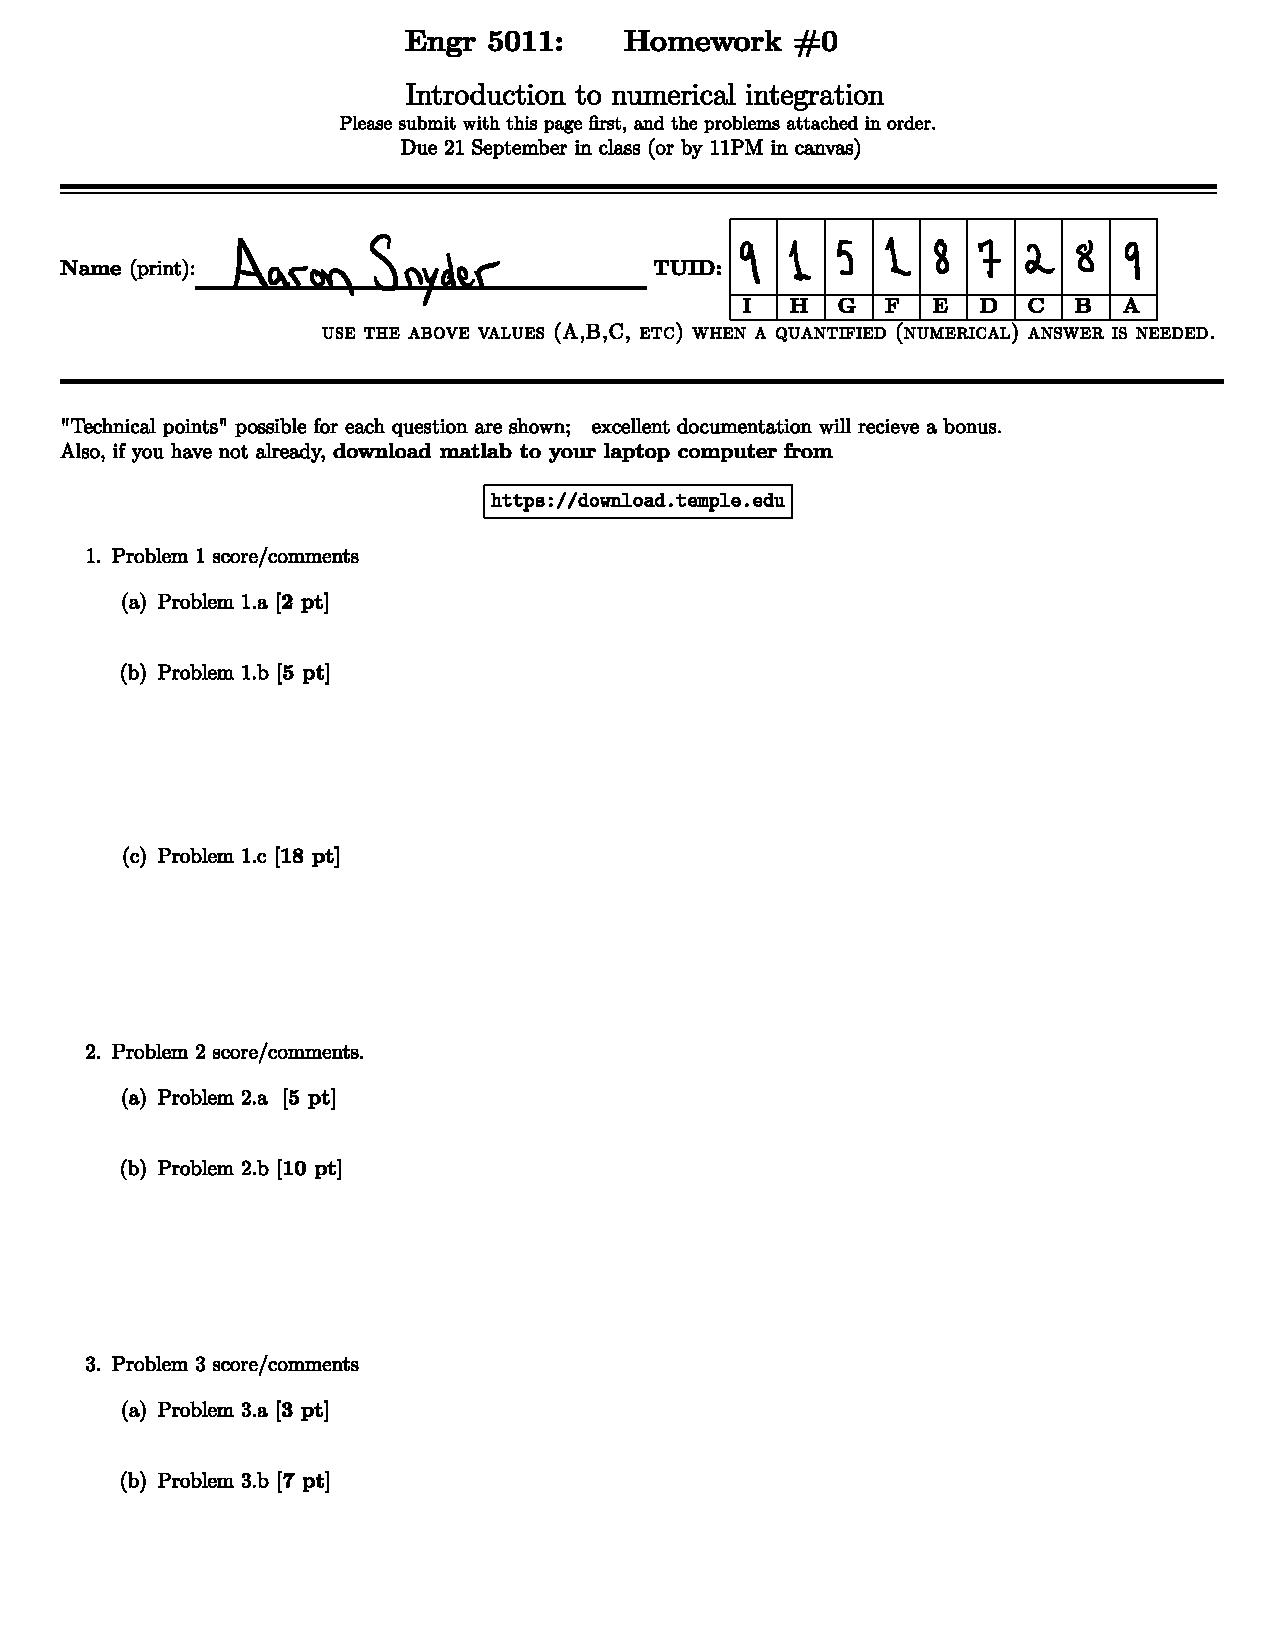
\includepdf[pages=-]{hw0_cover.pdf} % Include the Python PDF

\section{Hand Calcs}
\begin{figure}[h]
    \centering
    
\includegraphics[width=1\textwidth]{hand-calcs.jpg}
\end{figure}

\vspace{2cm}  % Add vertical space of 2cm

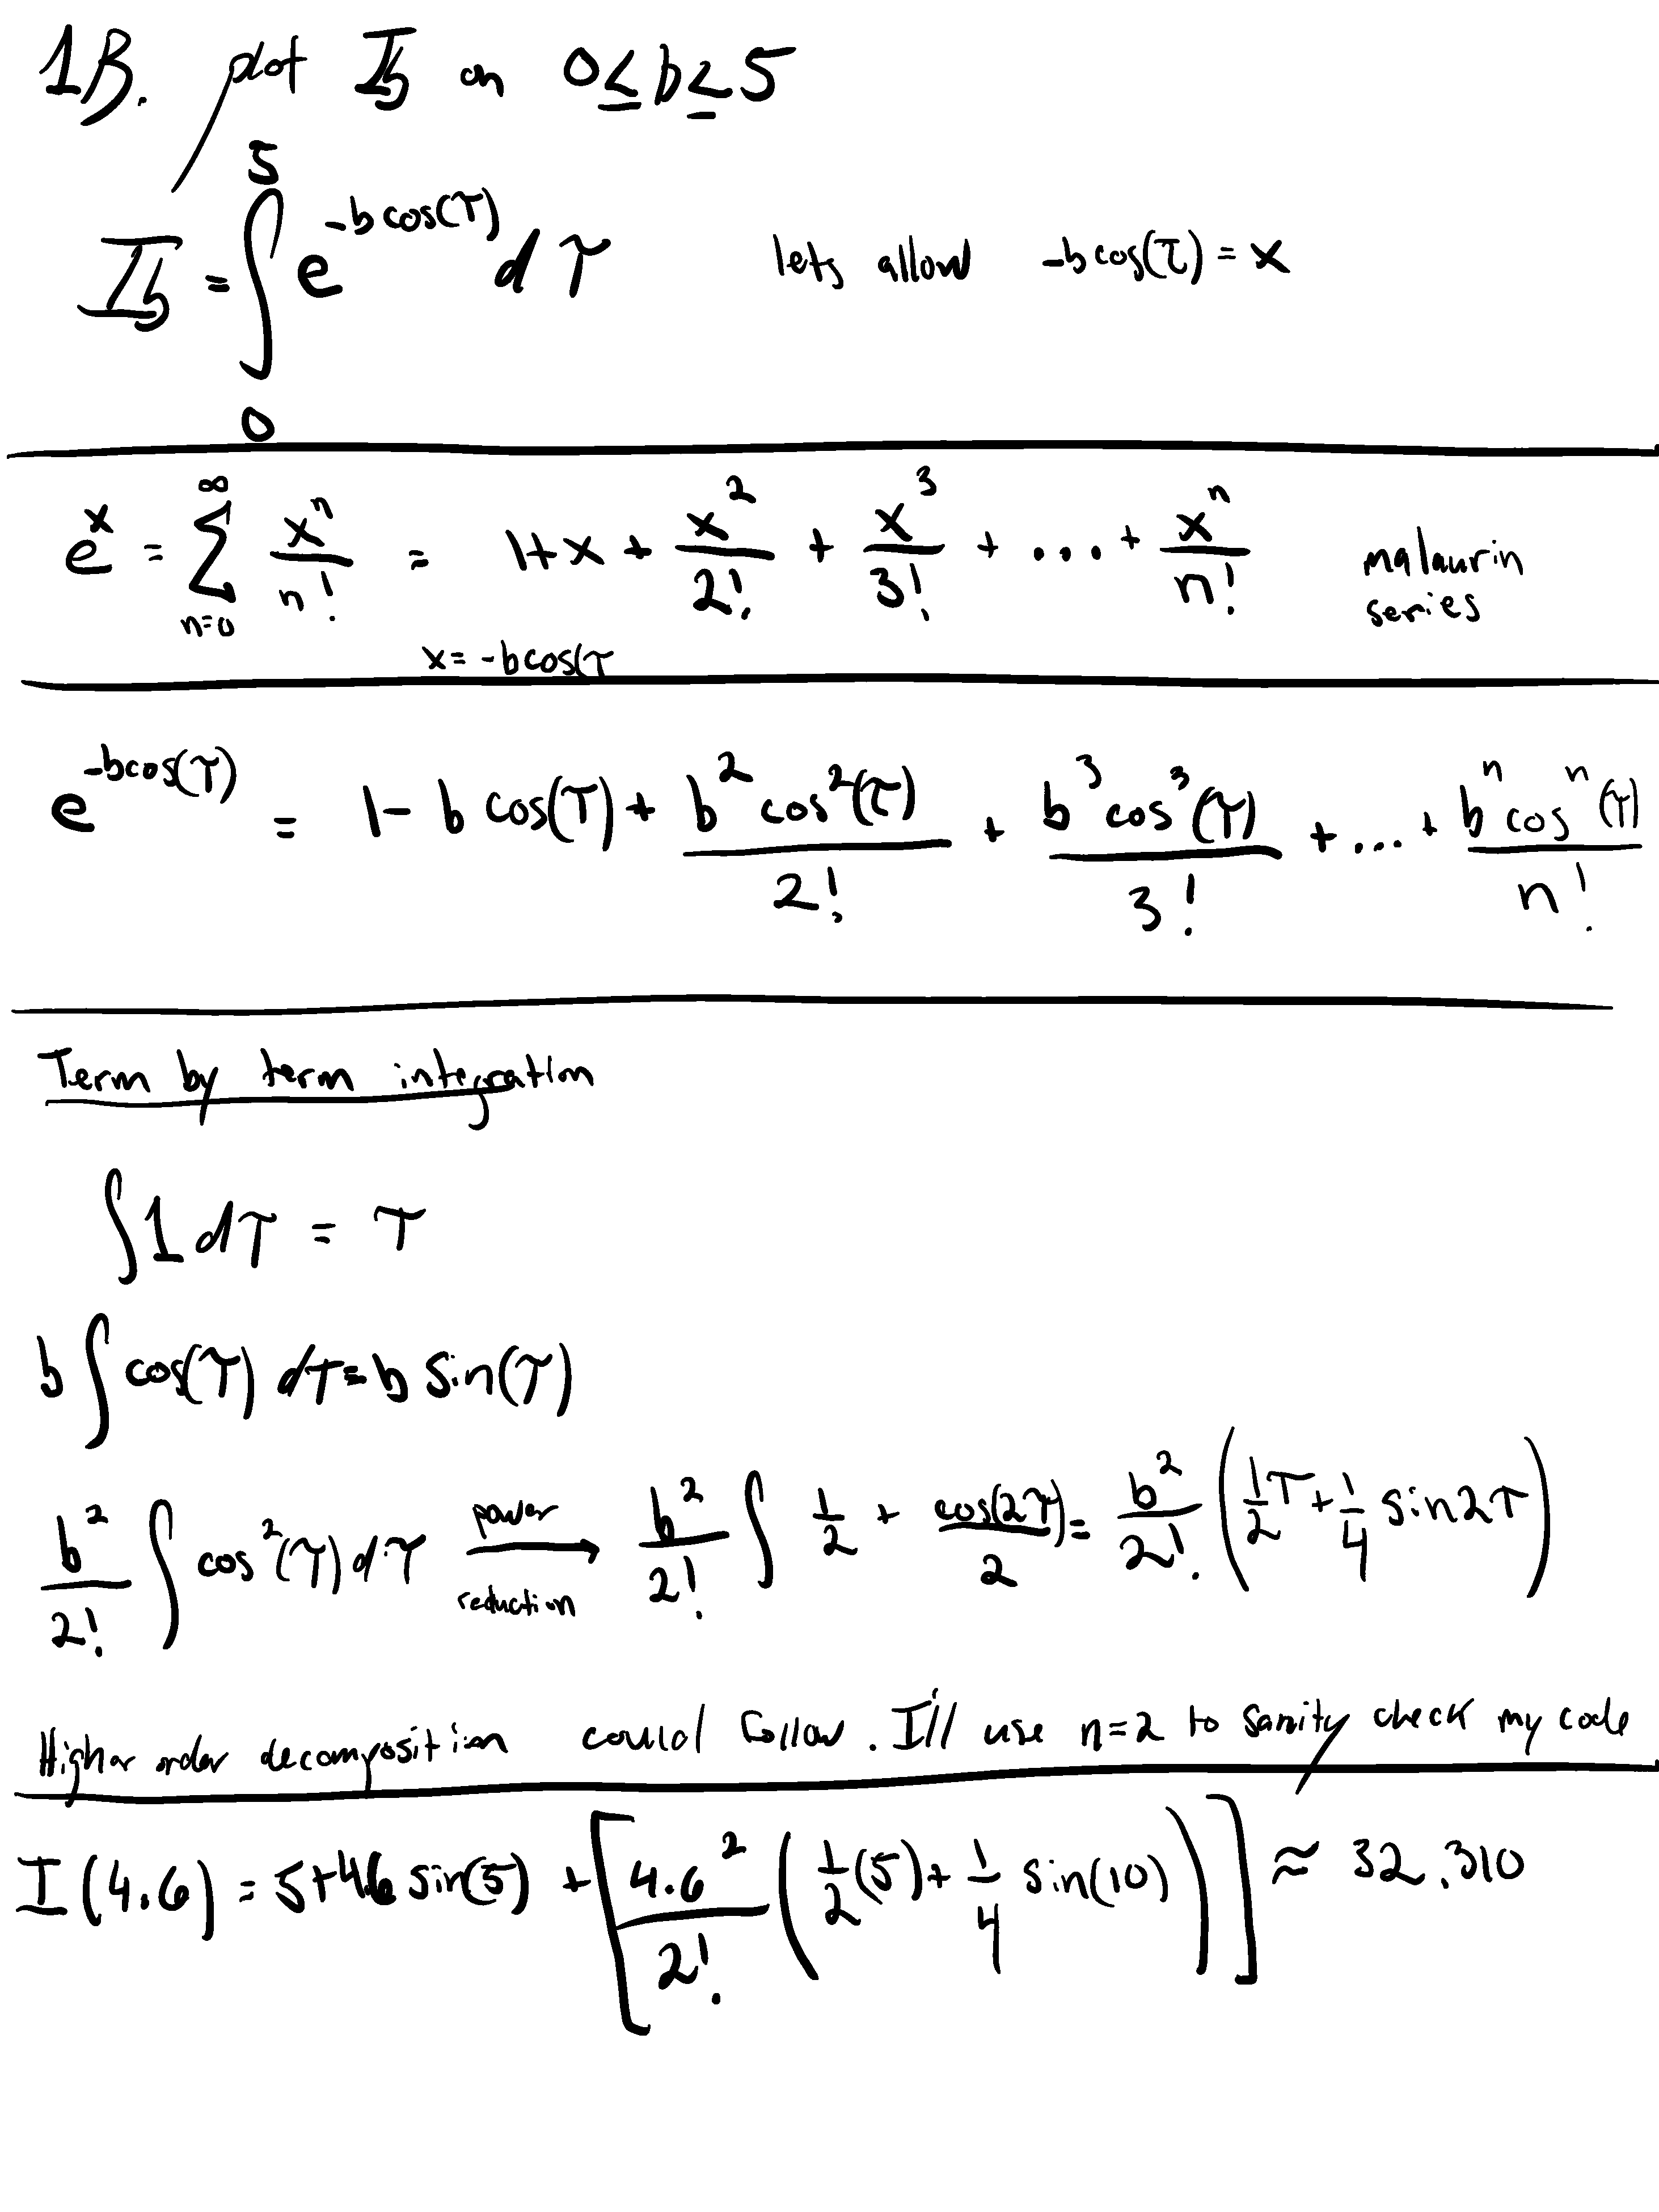
\includepdf[pages=-]{hand_calcs/1b.pdf} % Include the Python PDF
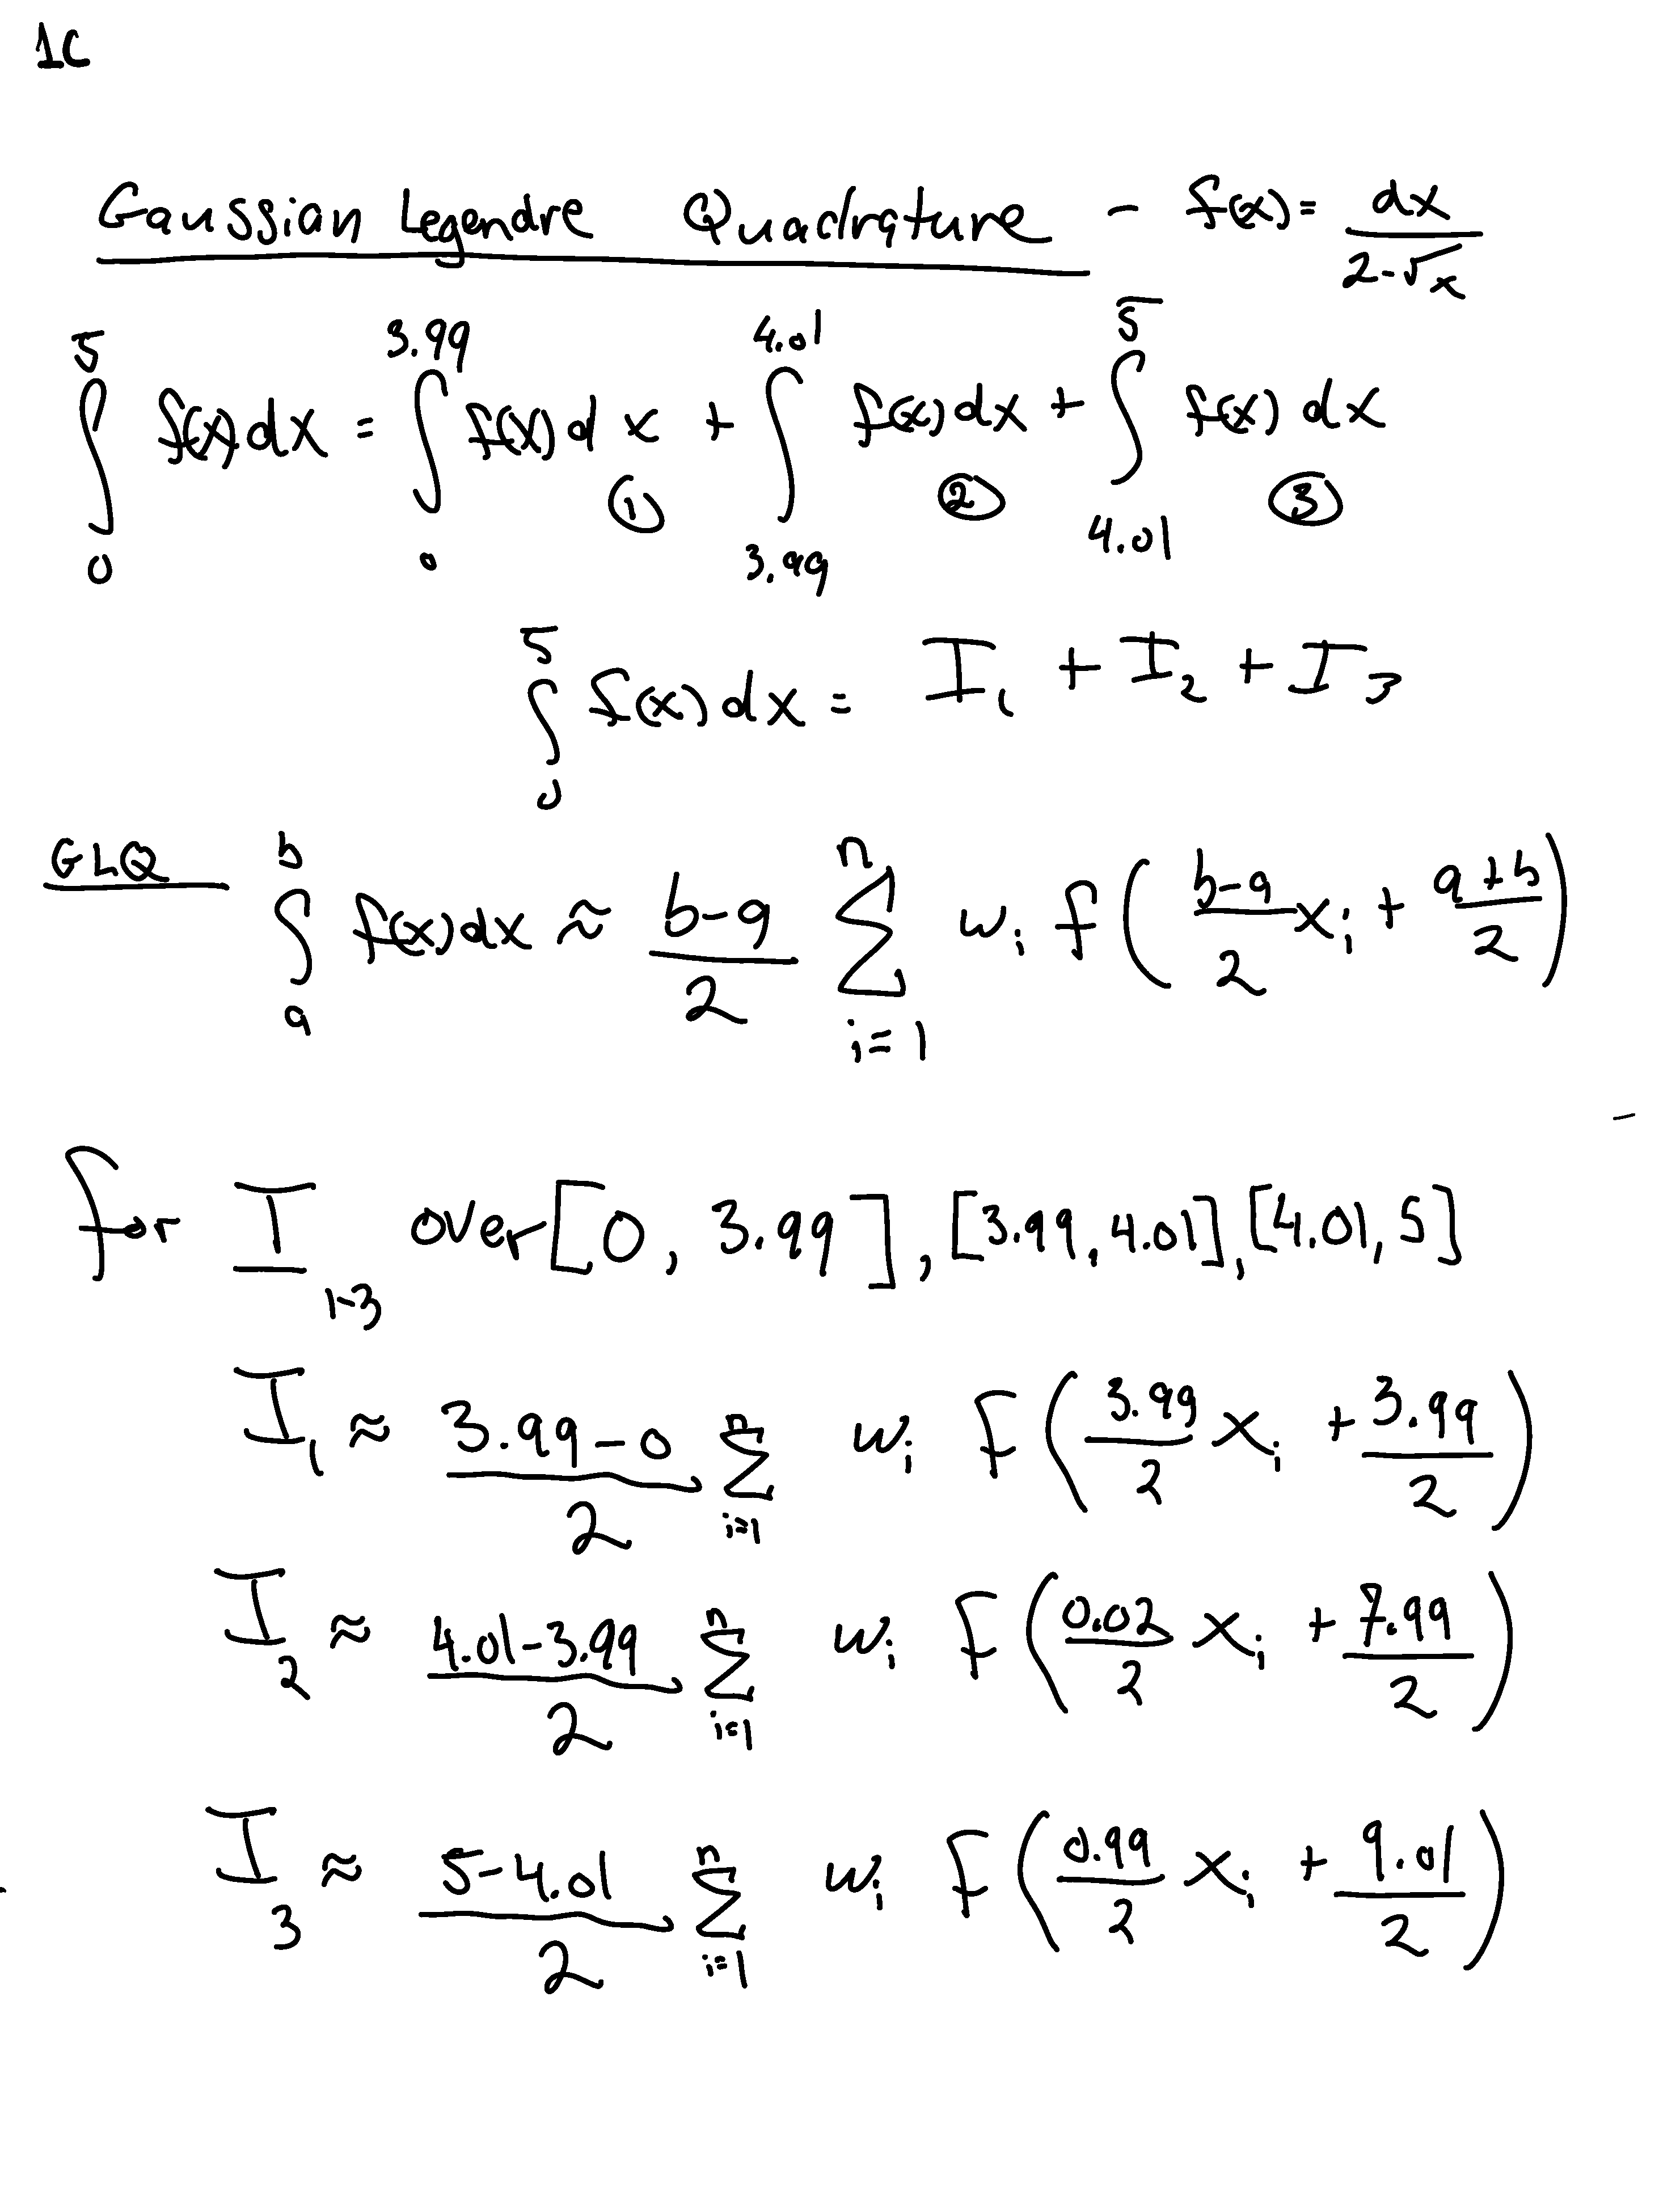
\includepdf[pages=-]{hand_calcs/1c.pdf} % Include the Python PDF
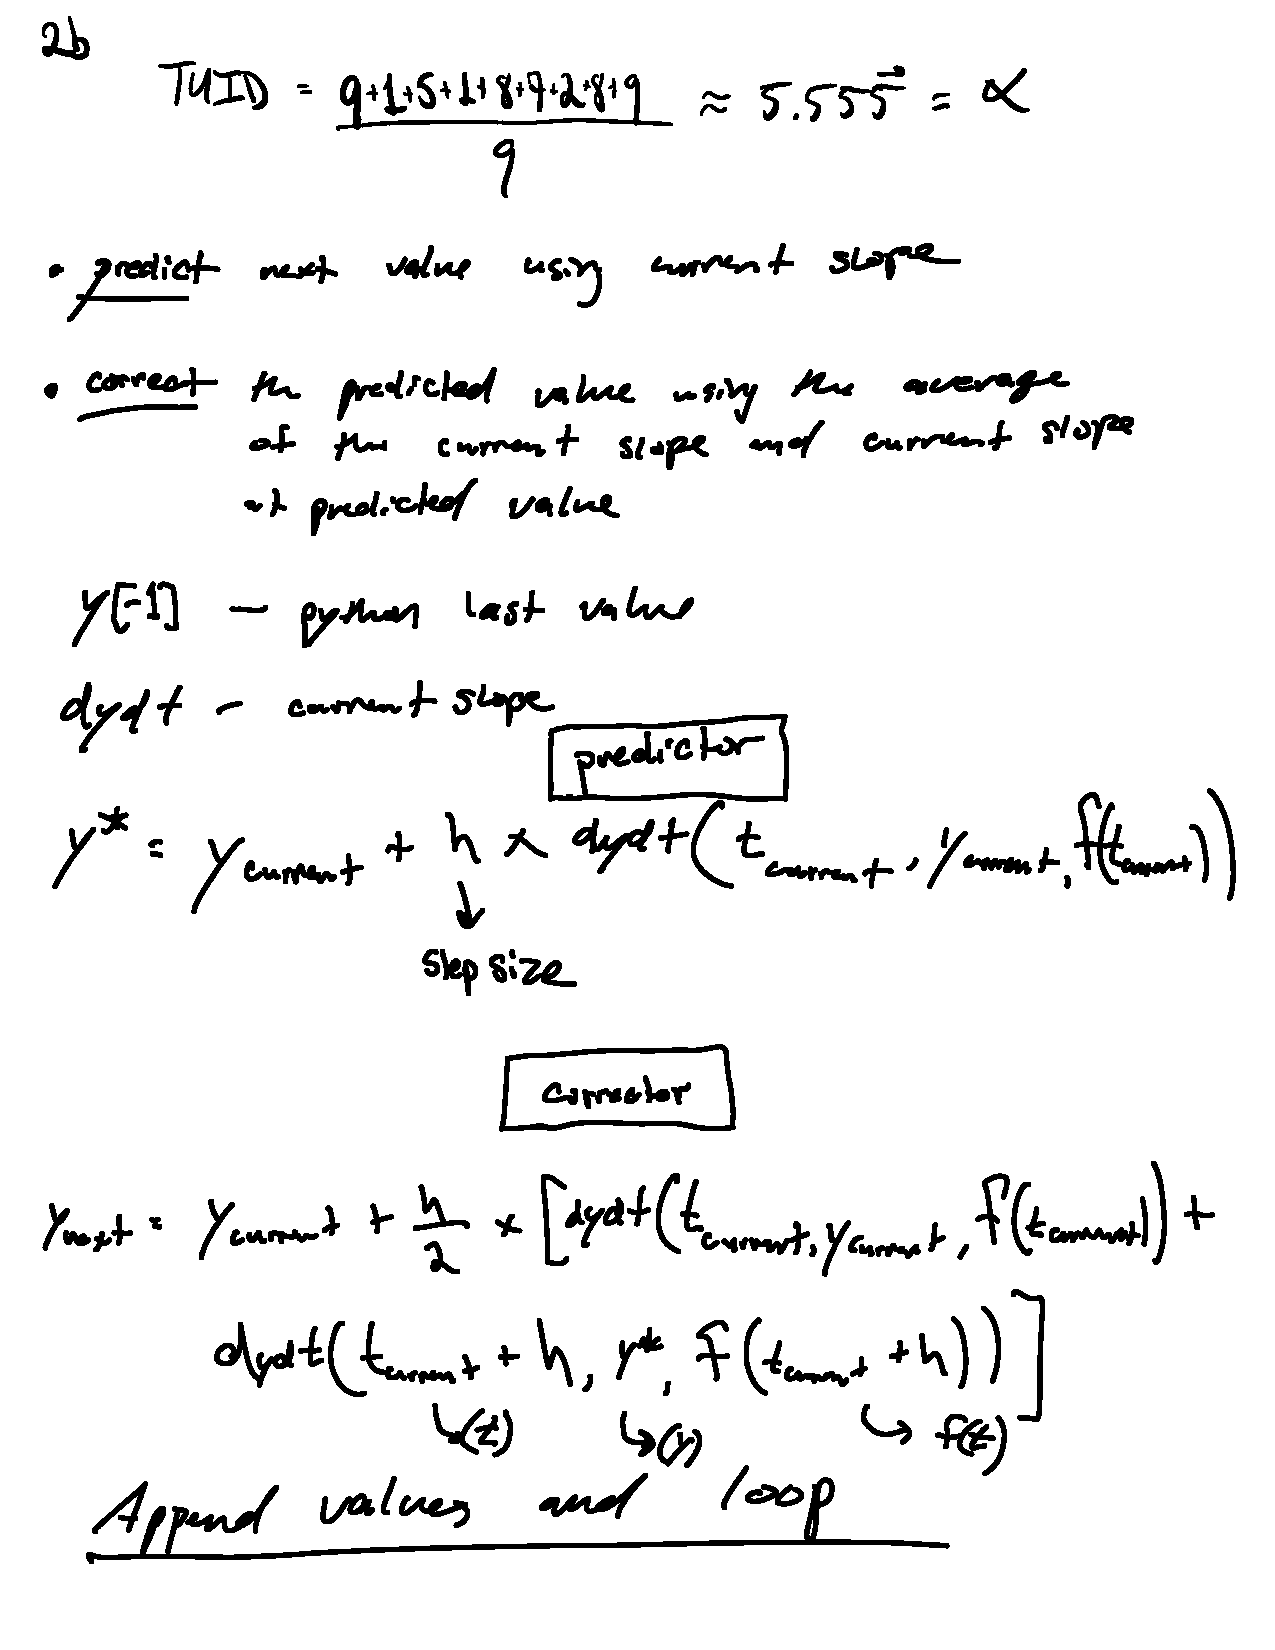
\includepdf[pages=-]{hand_calcs/2b.pdf} % Include the Python PDF
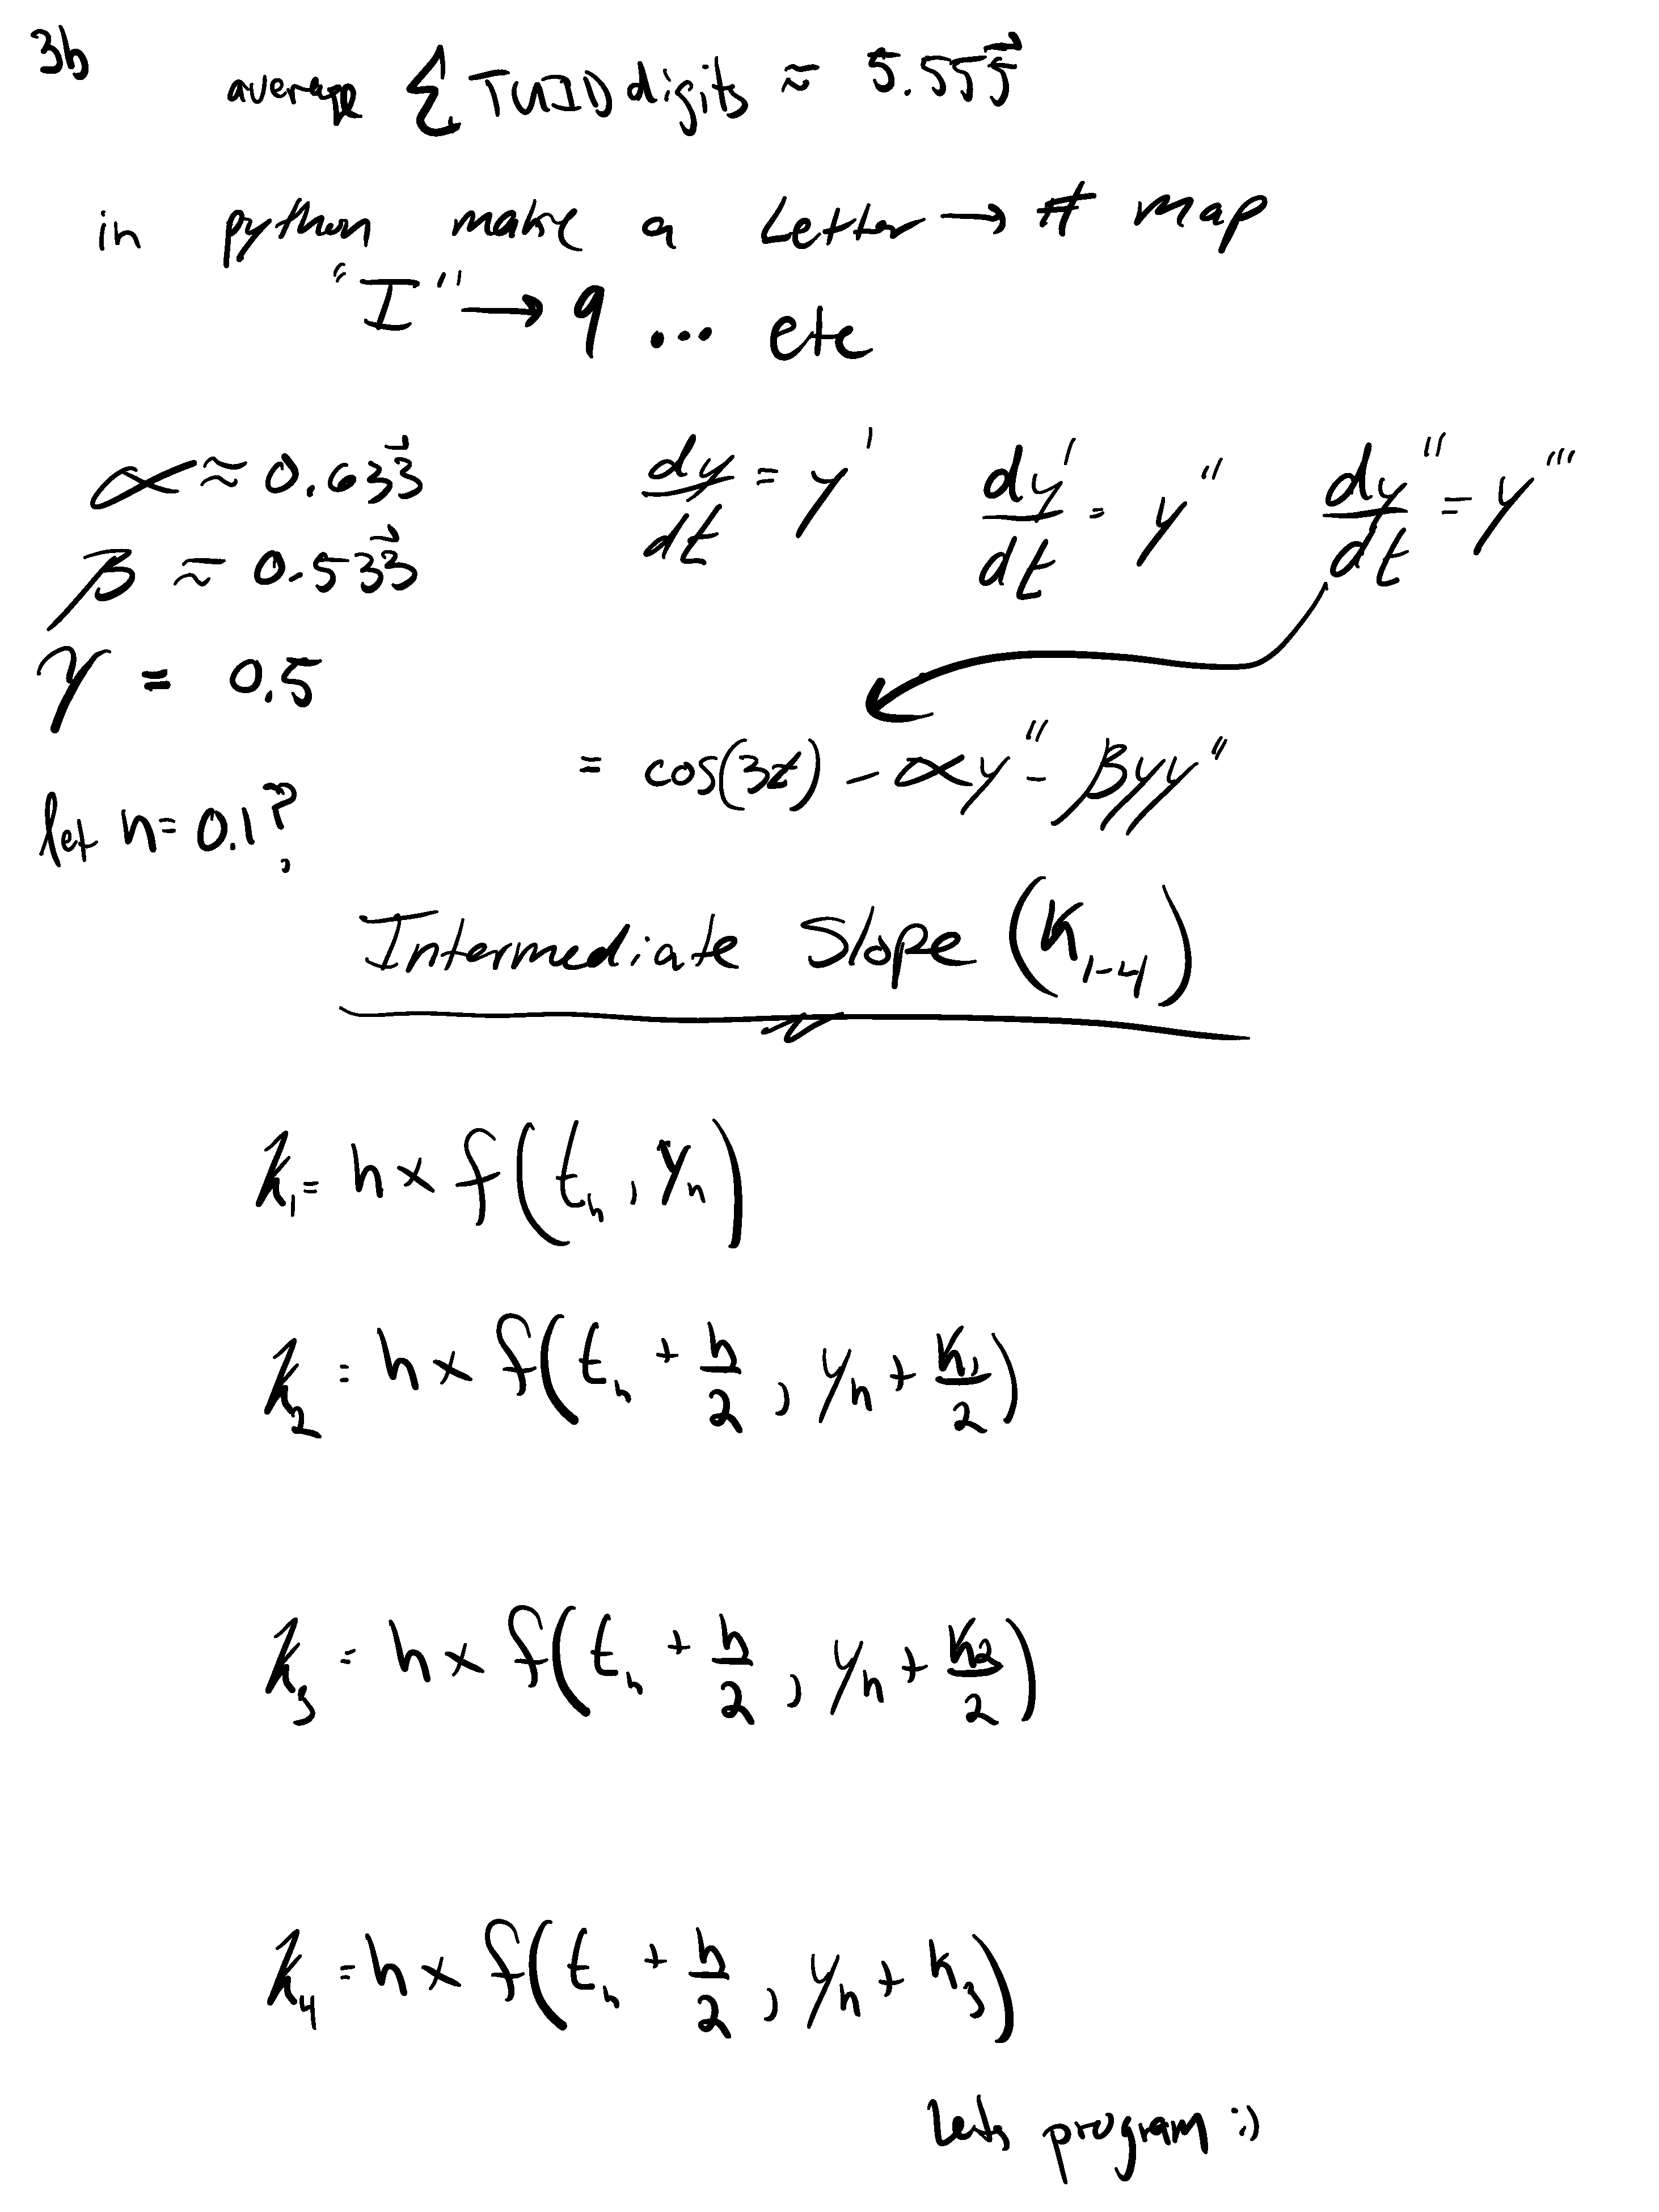
\includepdf[pages=-]{hand_calcs/3b.pdf} % Include the Python PDF


\section{Python Outputs}
\begin{figure}[h]
    \centering
    
\includegraphics[width=0.5\textwidth]{Python-Logo.jpg}
\end{figure}

\vspace{2cm}  % Add vertical space of 2cm

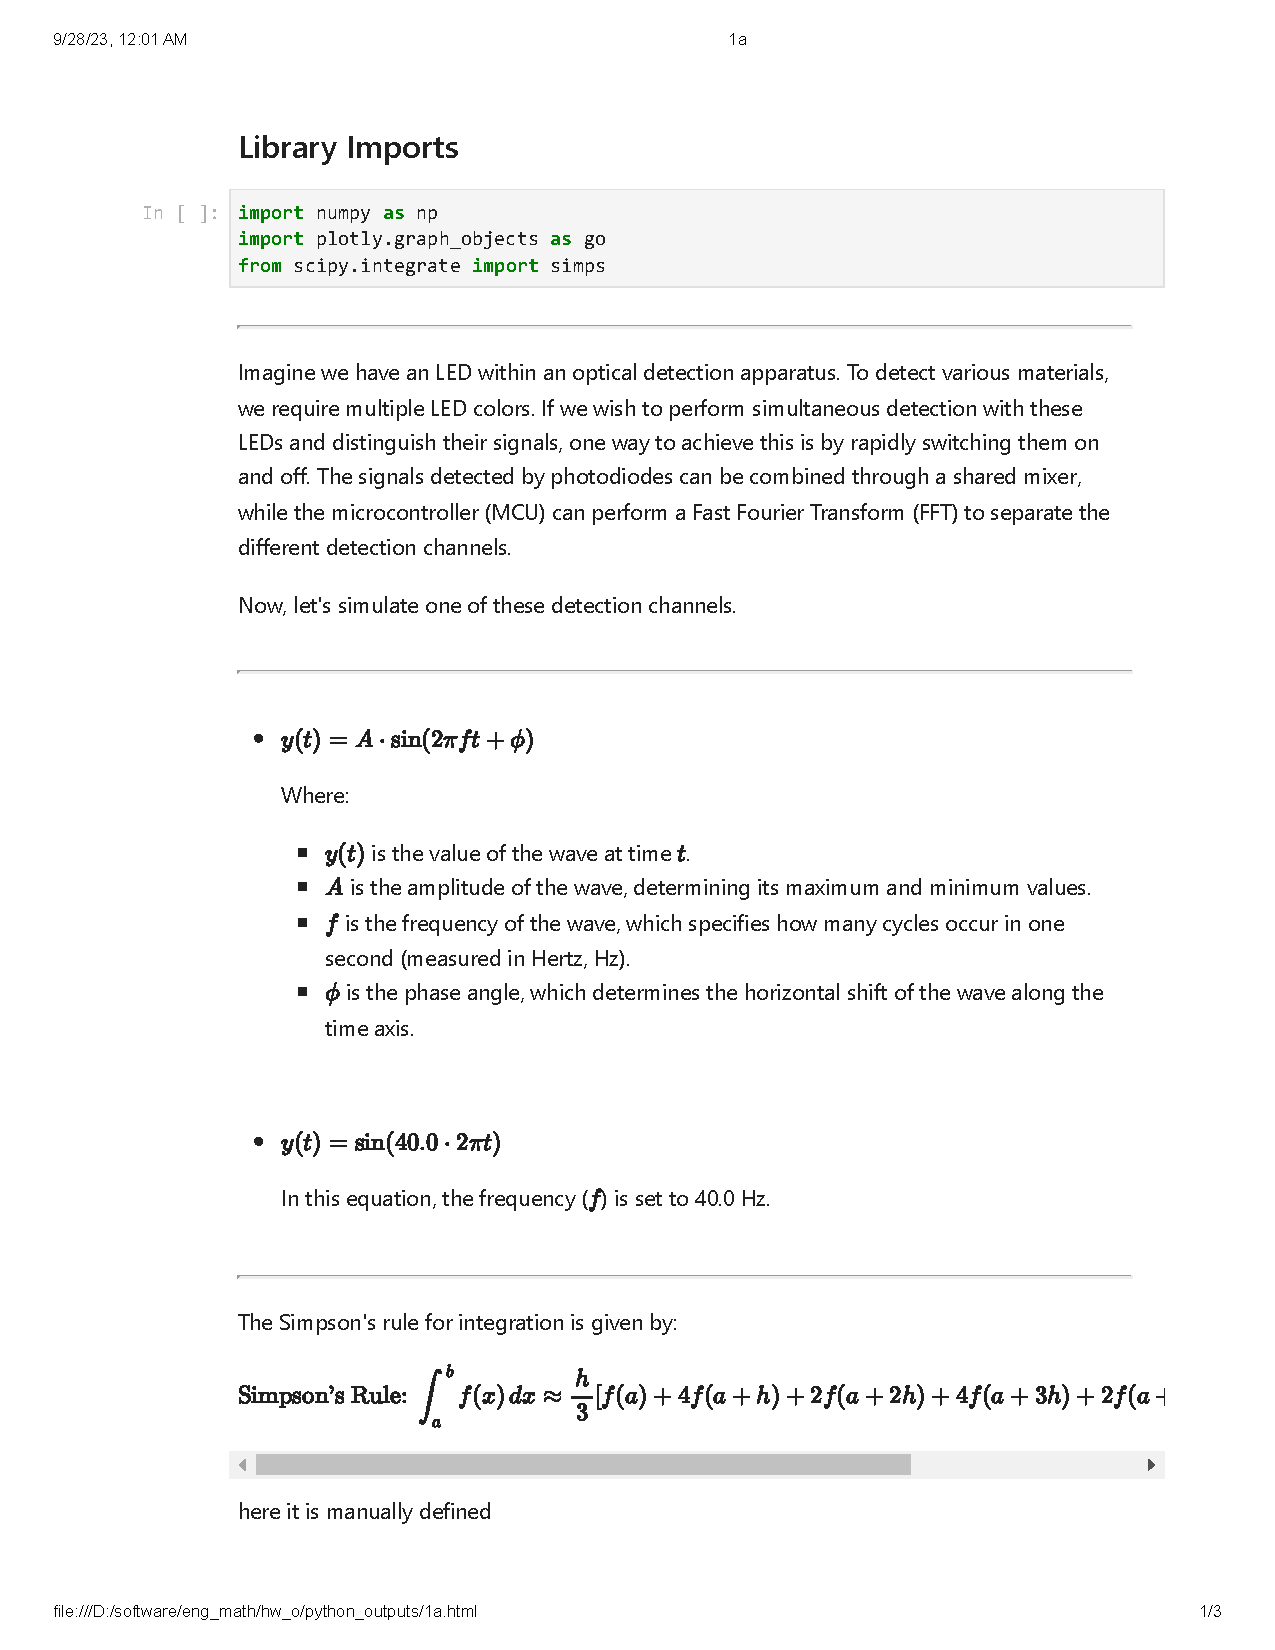
\includepdf[pages=-]{python_outputs/1a.pdf} % Include the Python PDF
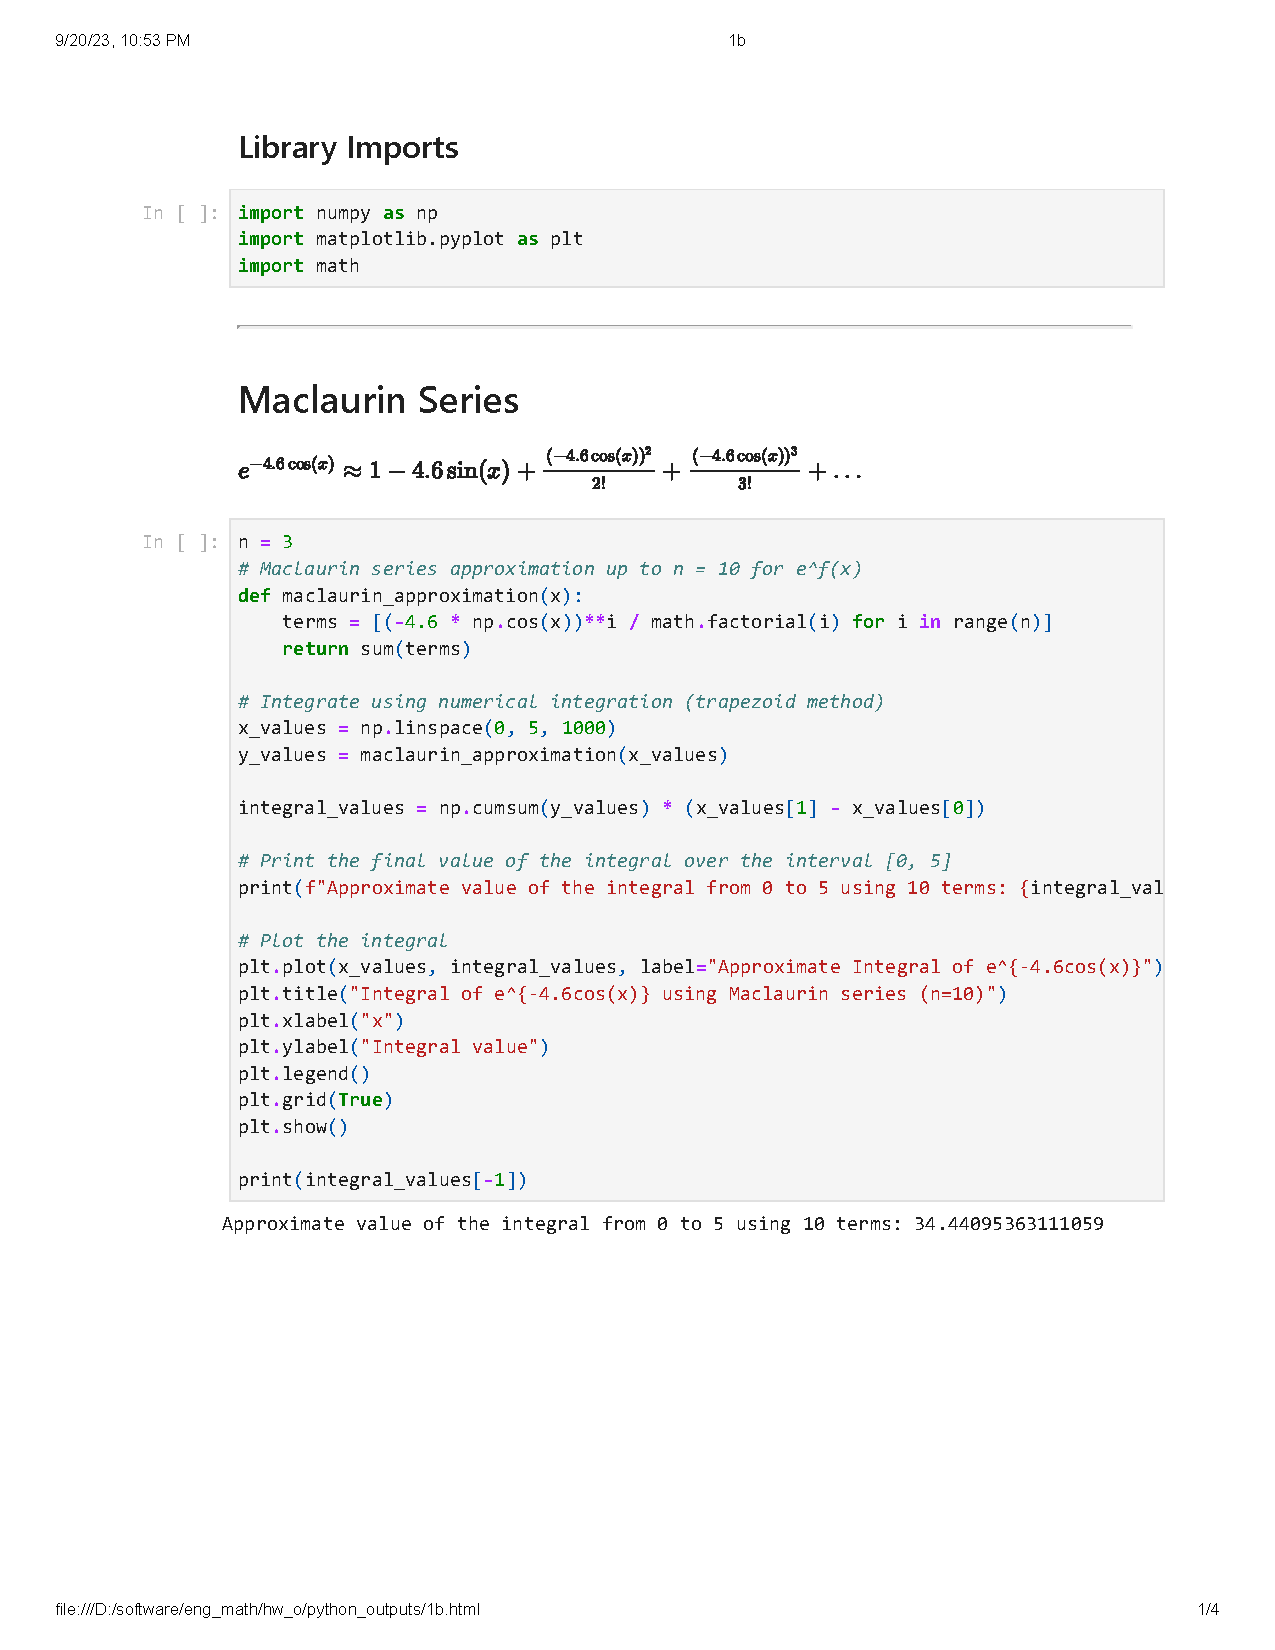
\includepdf[pages=-]{python_outputs/1b.pdf} % Include the Python PDF
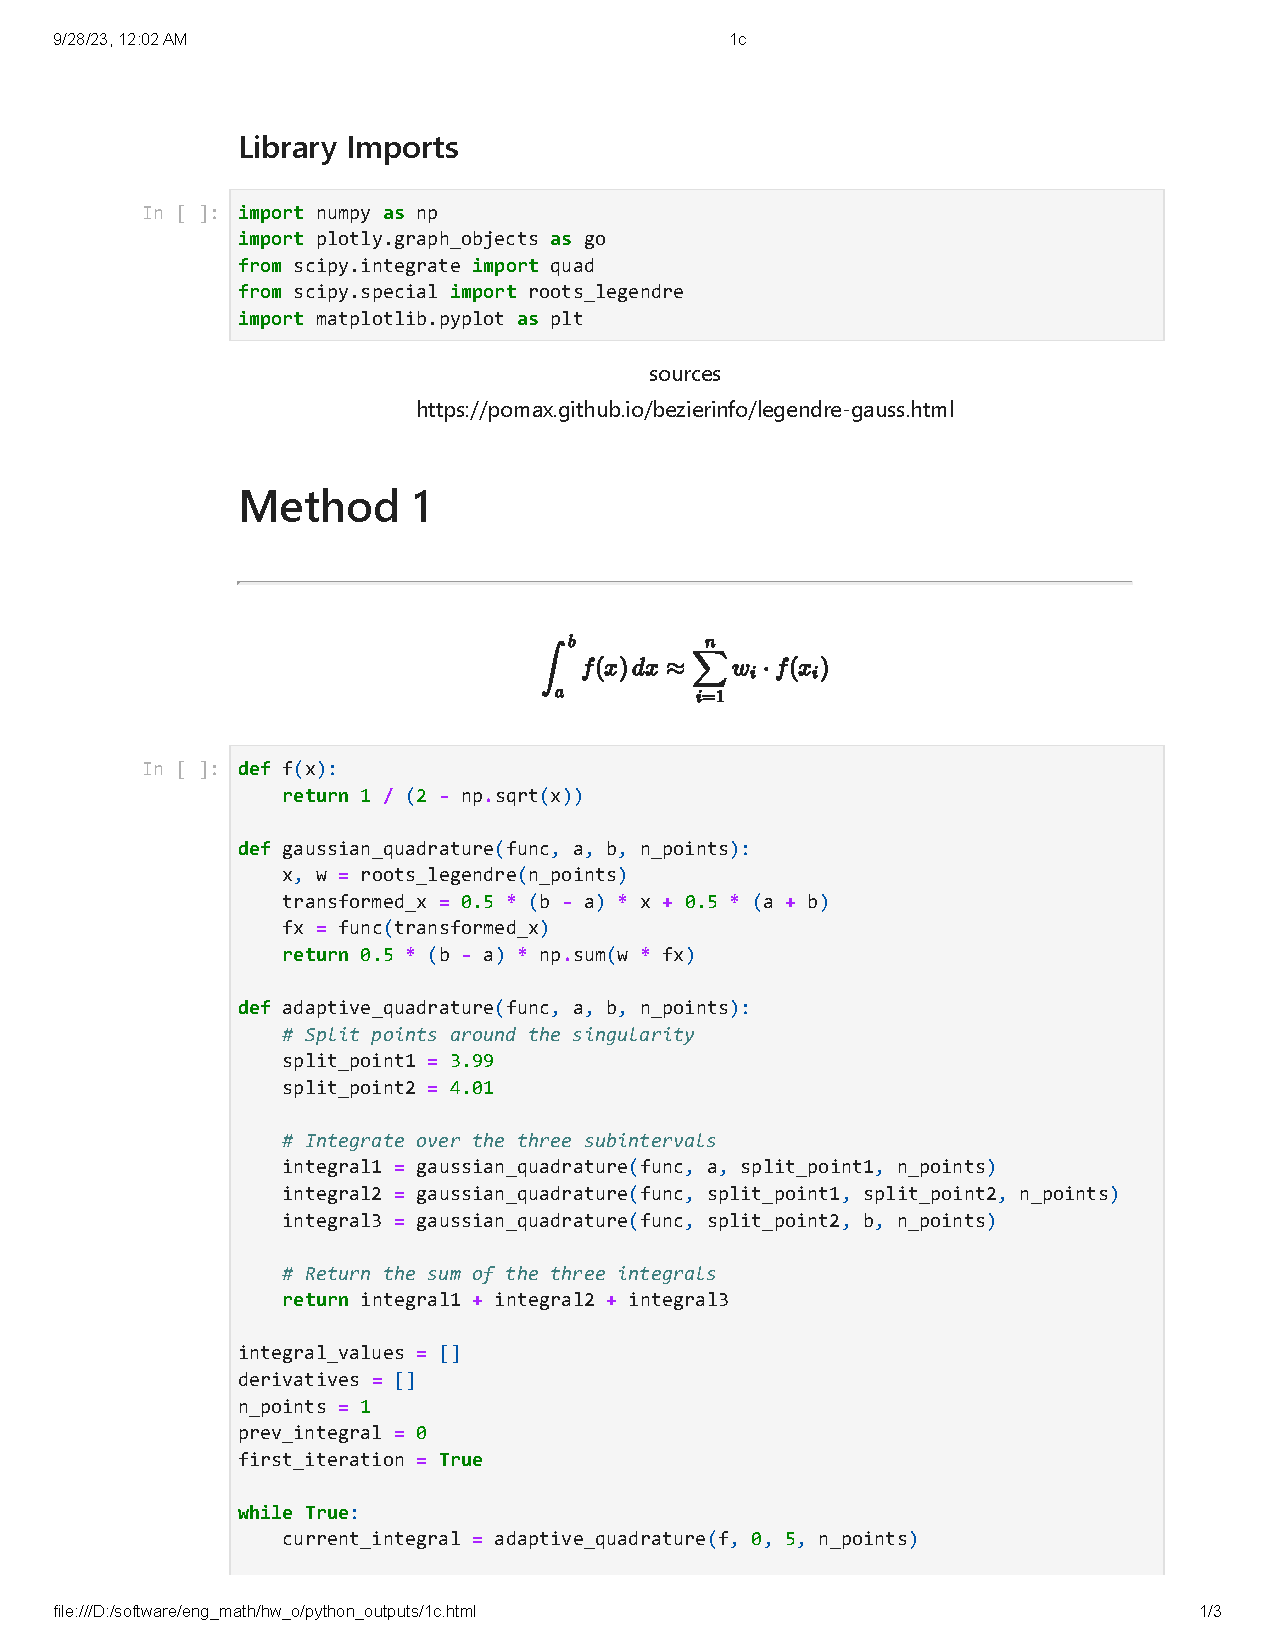
\includepdf[pages=-]{python_outputs/1c.pdf} % Include the Python PDF
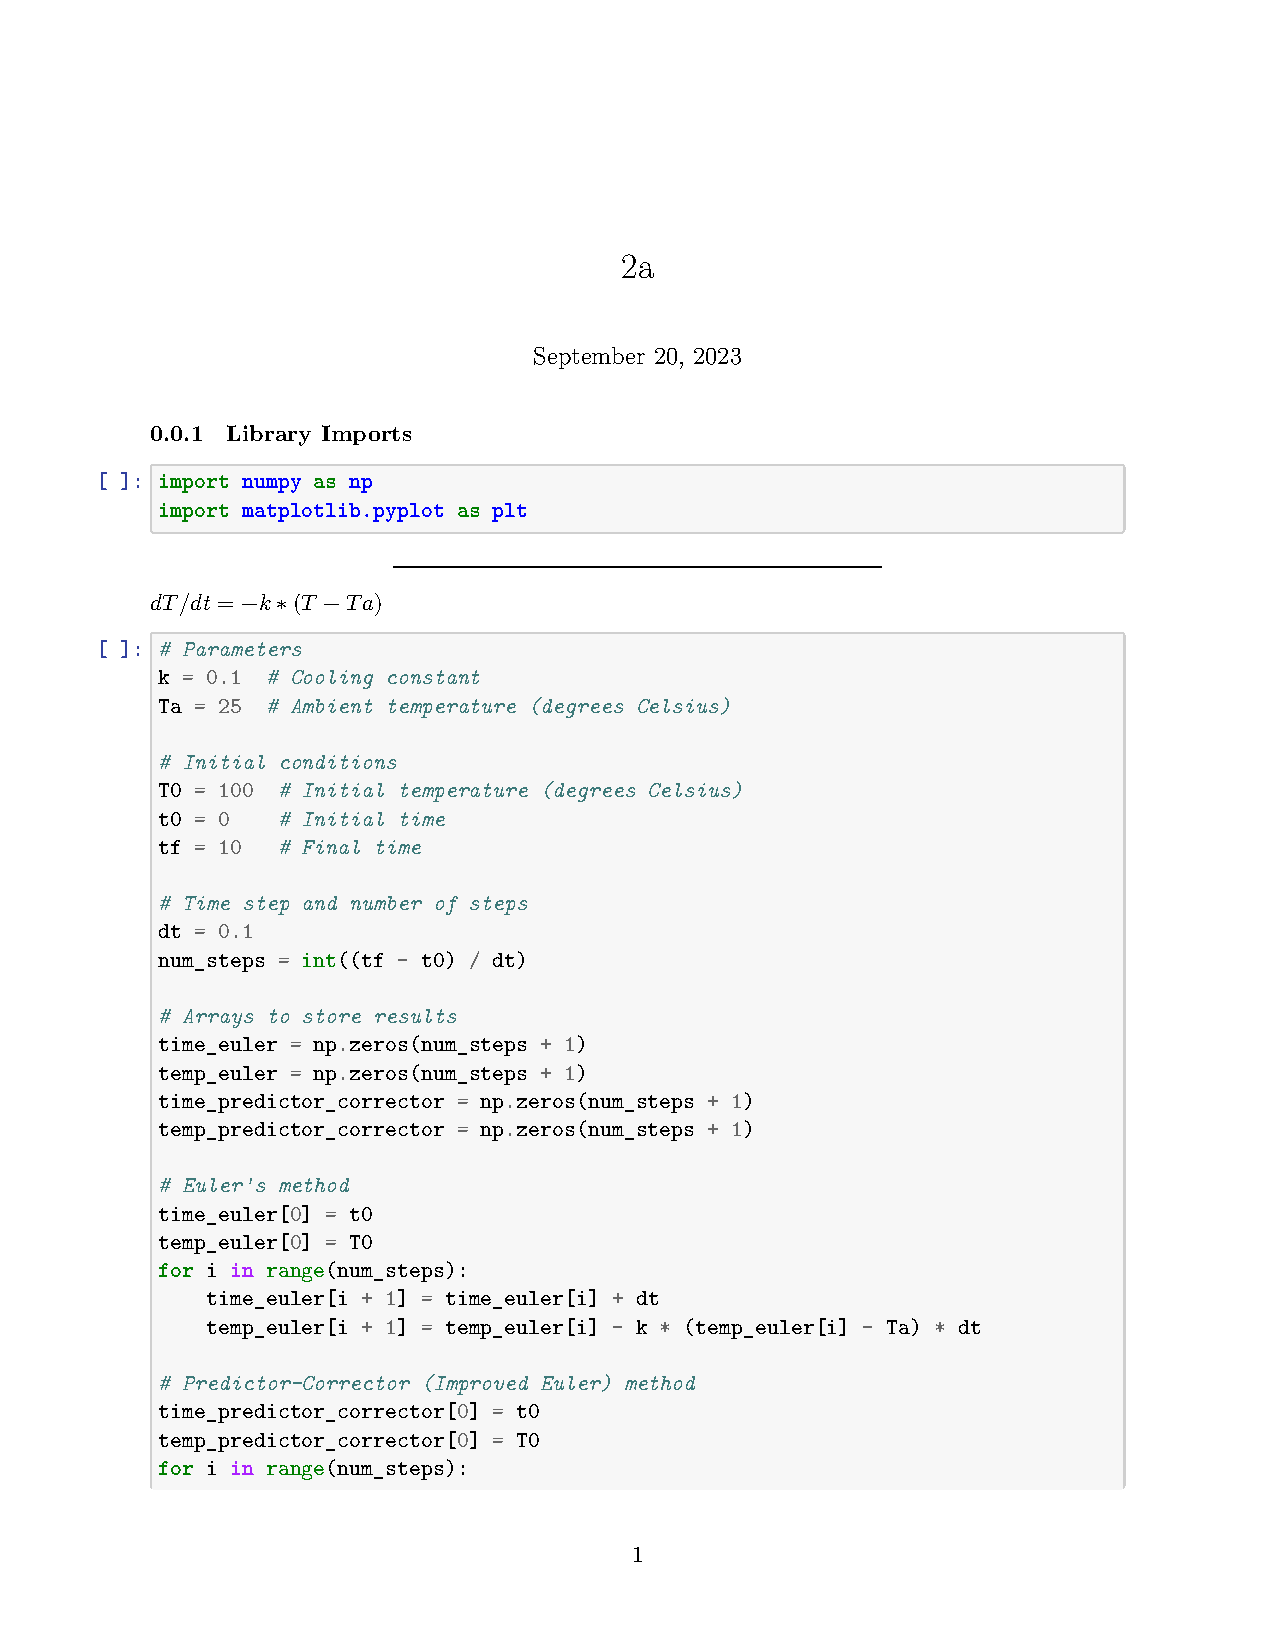
\includepdf[pages=-]{python_outputs/2a.pdf} % Include the Python PDF
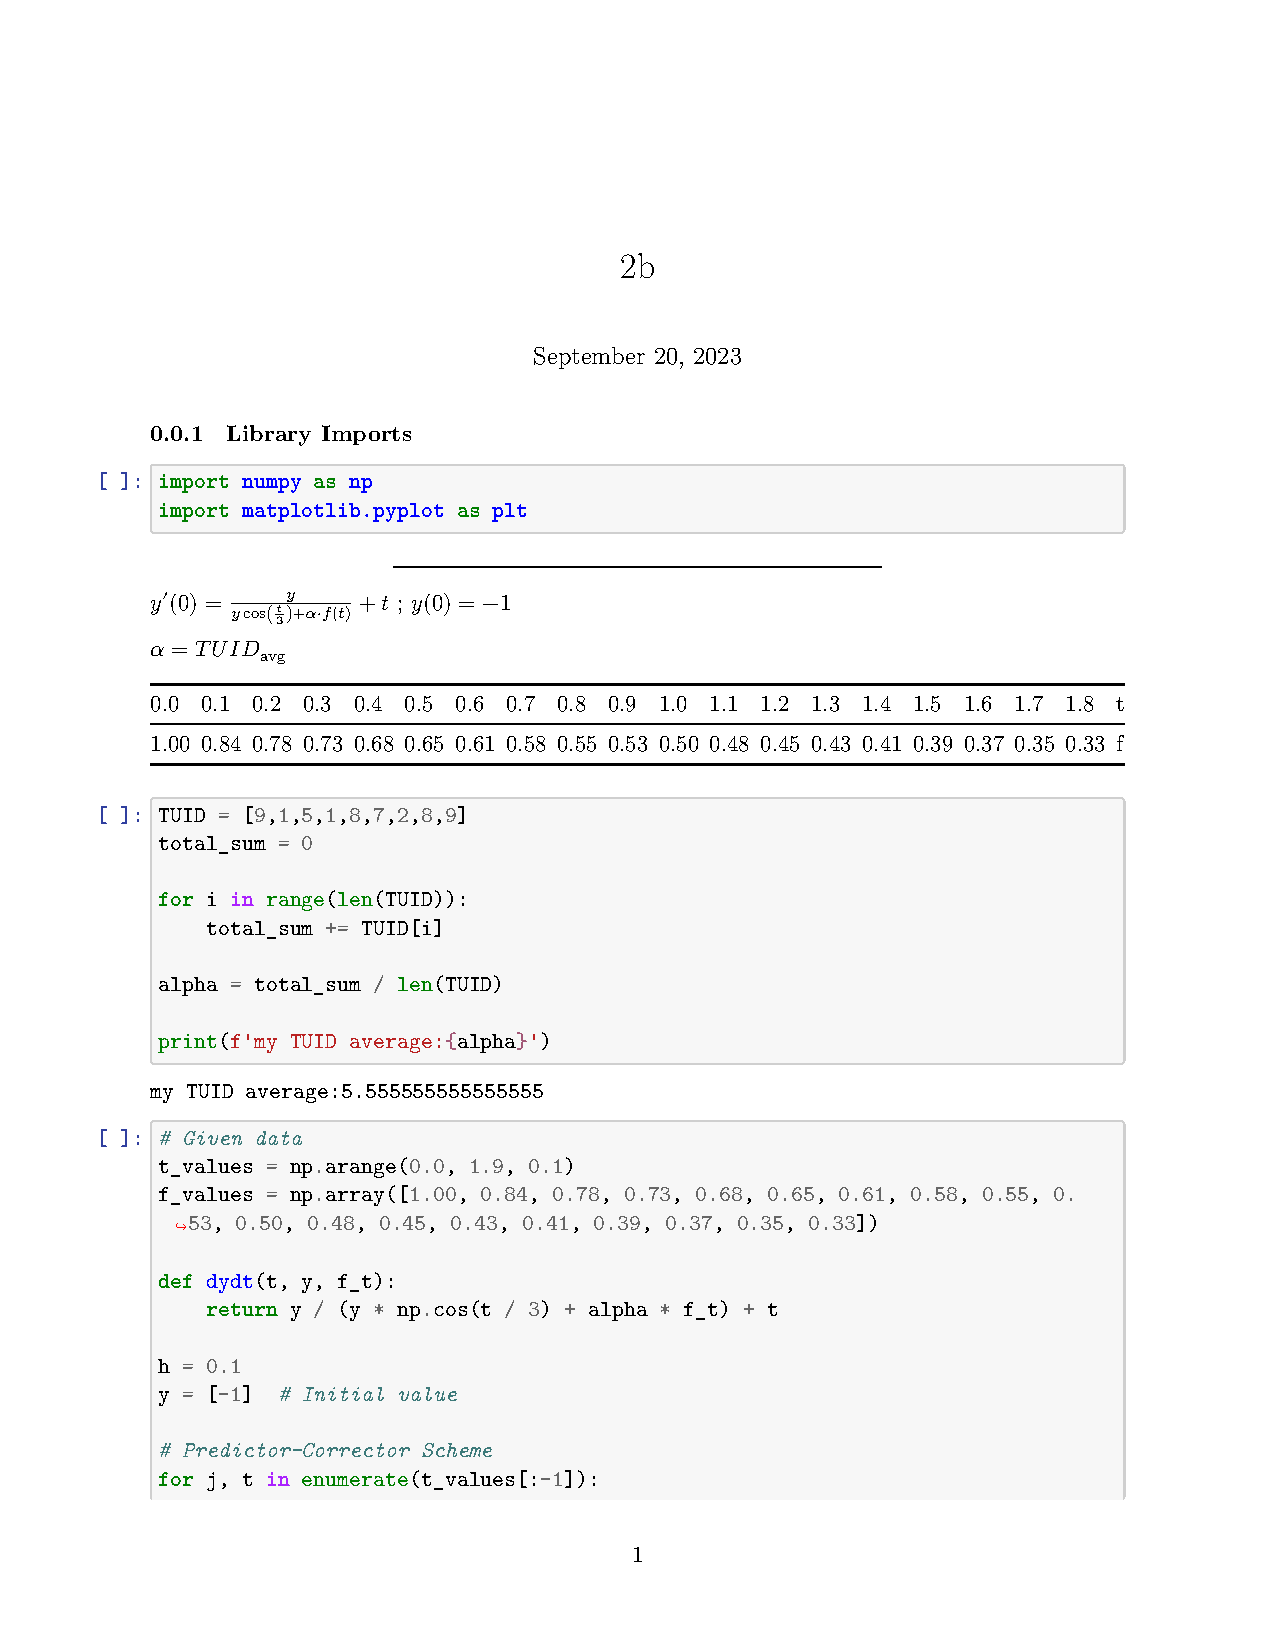
\includepdf[pages=-]{python_outputs/2b.pdf} % Include the Python PDF
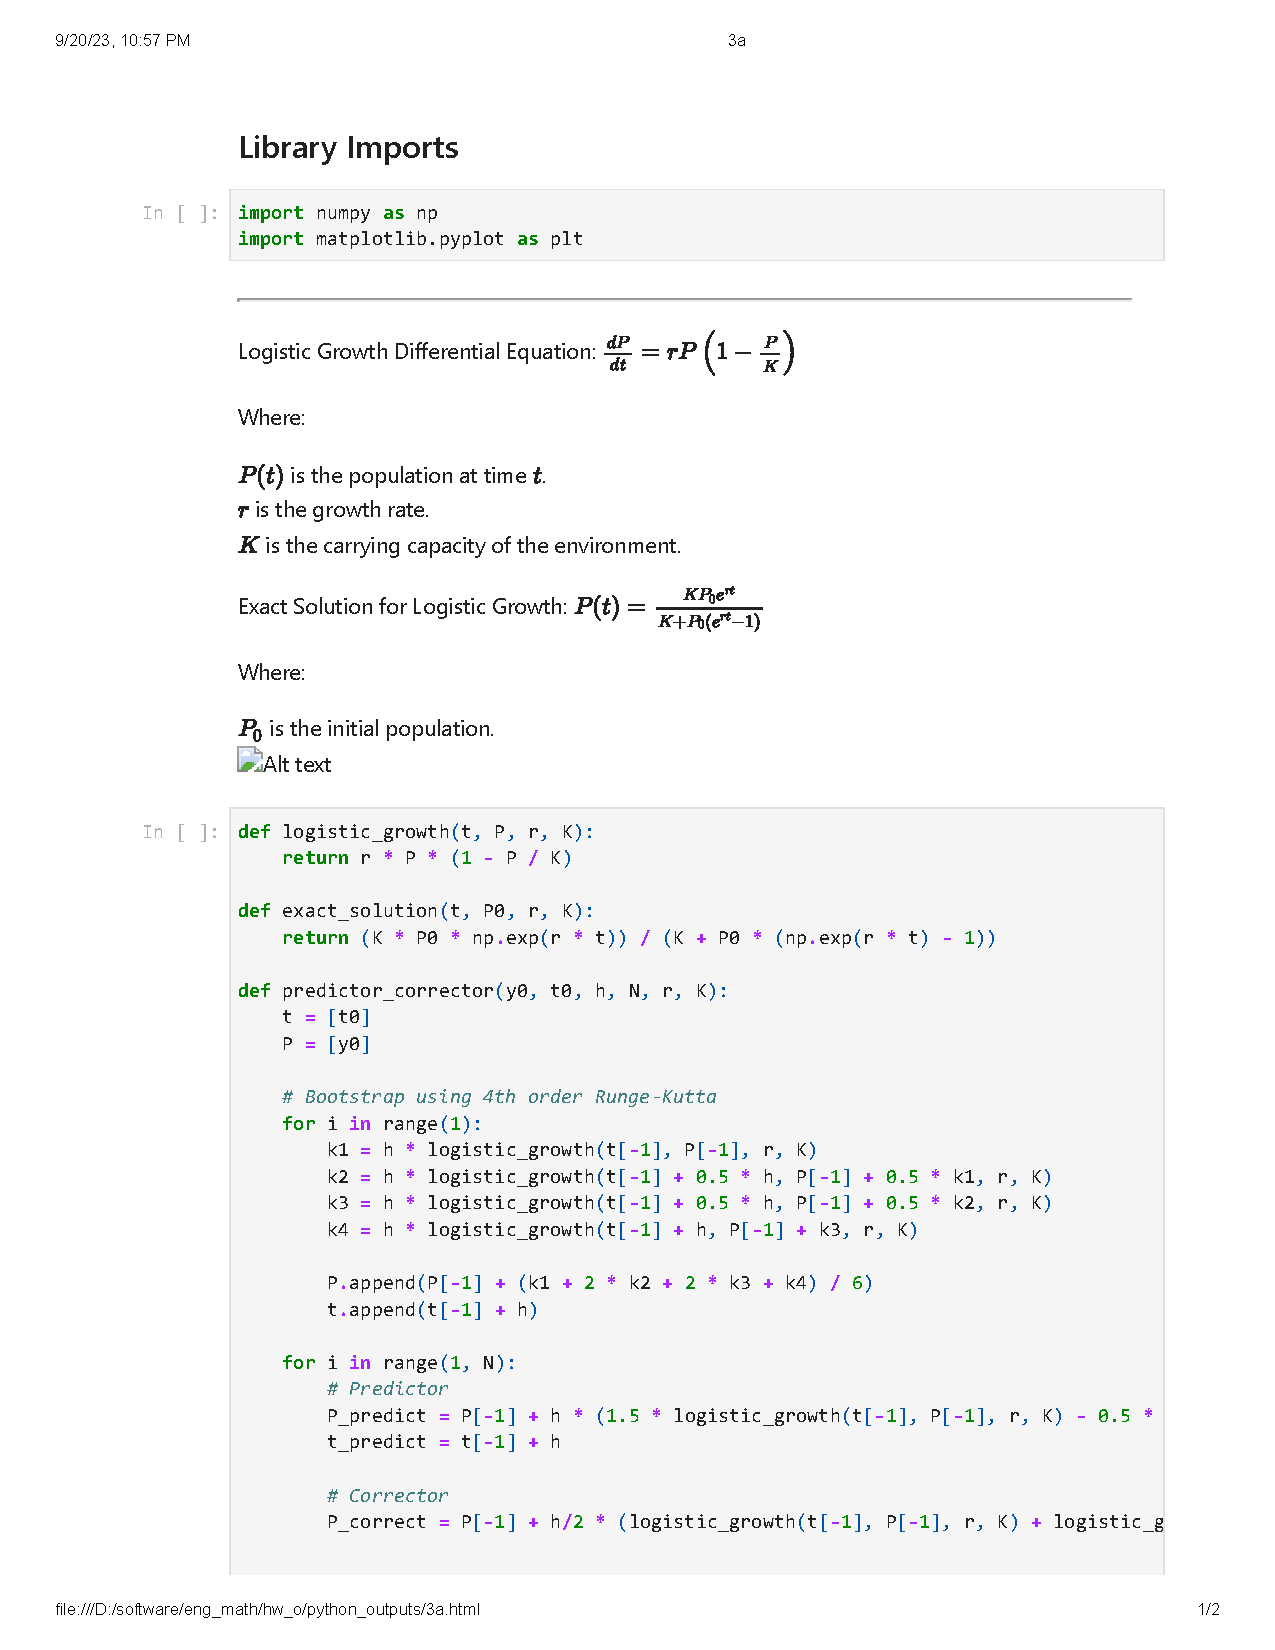
\includepdf[pages=-]{python_outputs/3a.pdf} % Include the Python PDF
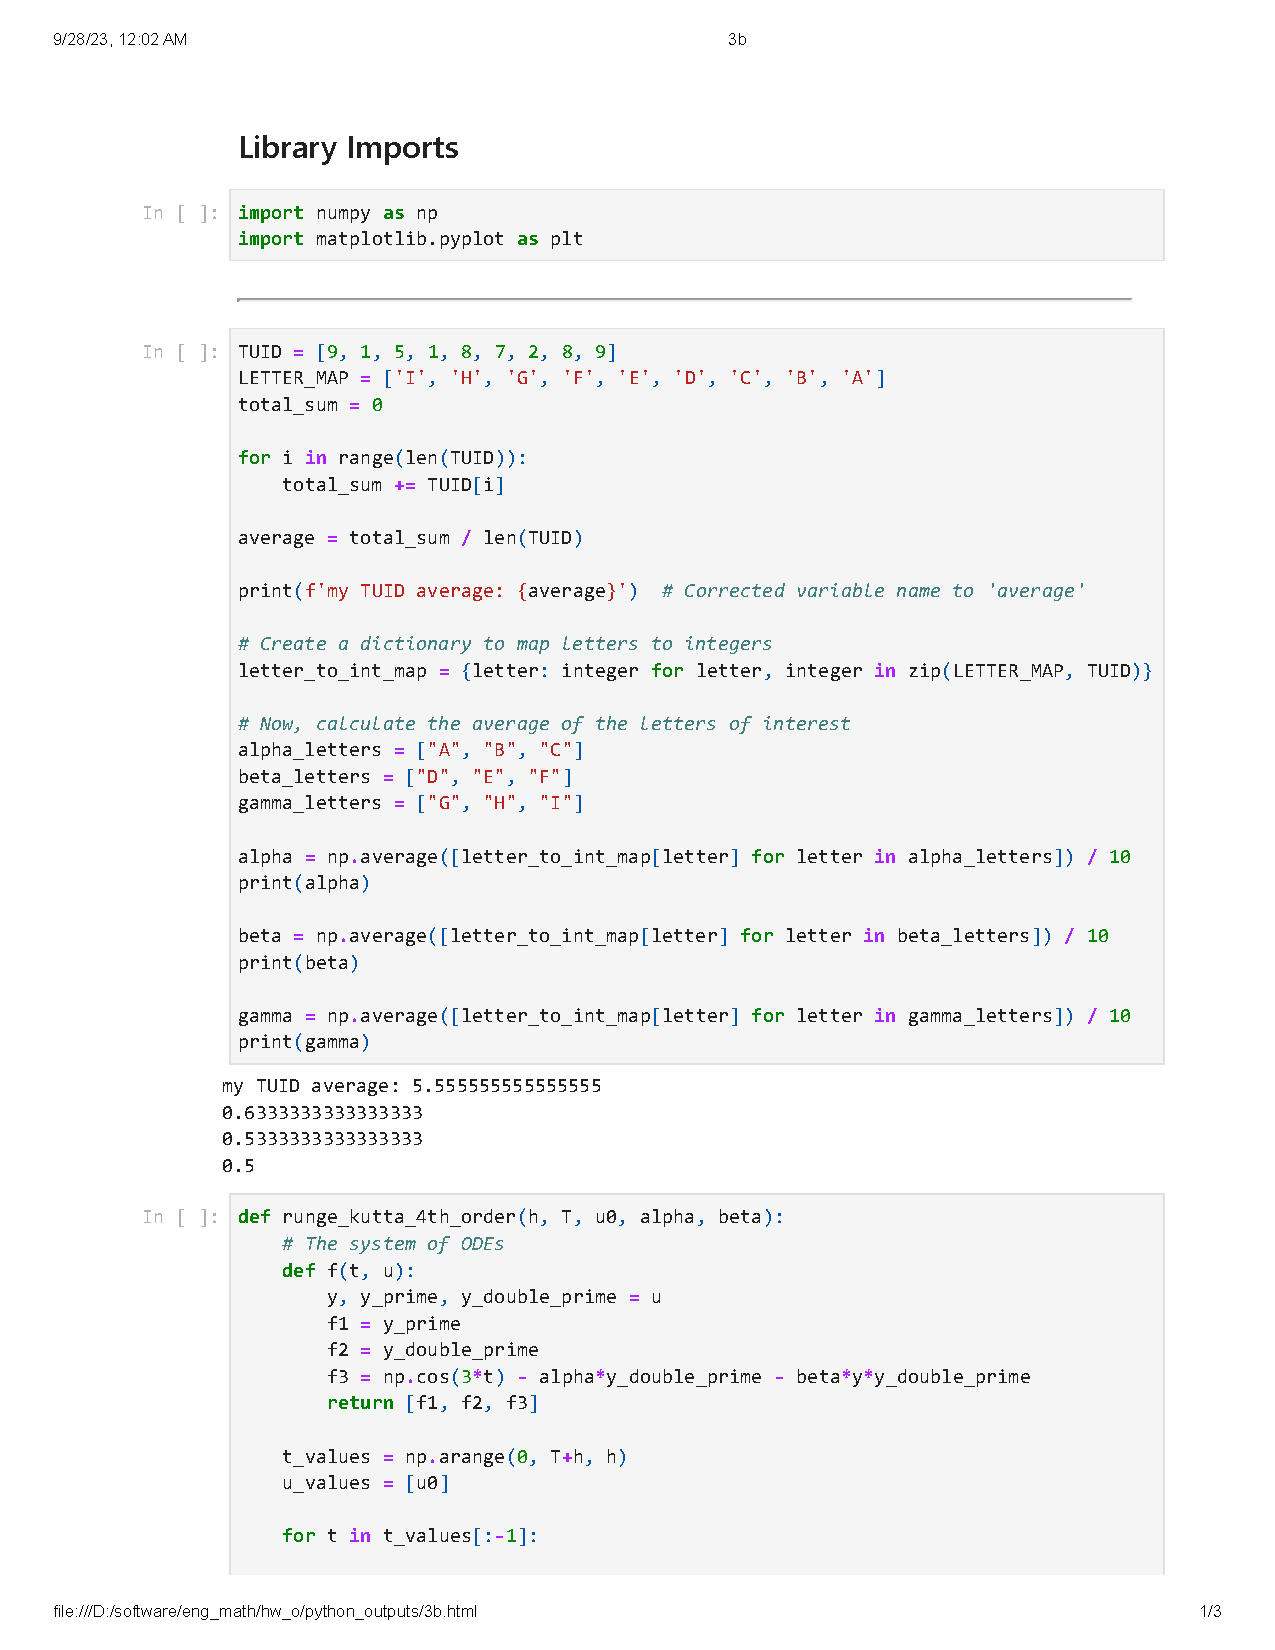
\includepdf[pages=-]{python_outputs/3b.pdf} % Include the Python PDF

\section{MATLAB Outputs}
\begin{figure}[h]
    \centering
    \includegraphics[width=0.5\textwidth]{Matlab-Logo.jpg}
\end{figure}

\vspace{2cm}  % Add vertical space of 2cm

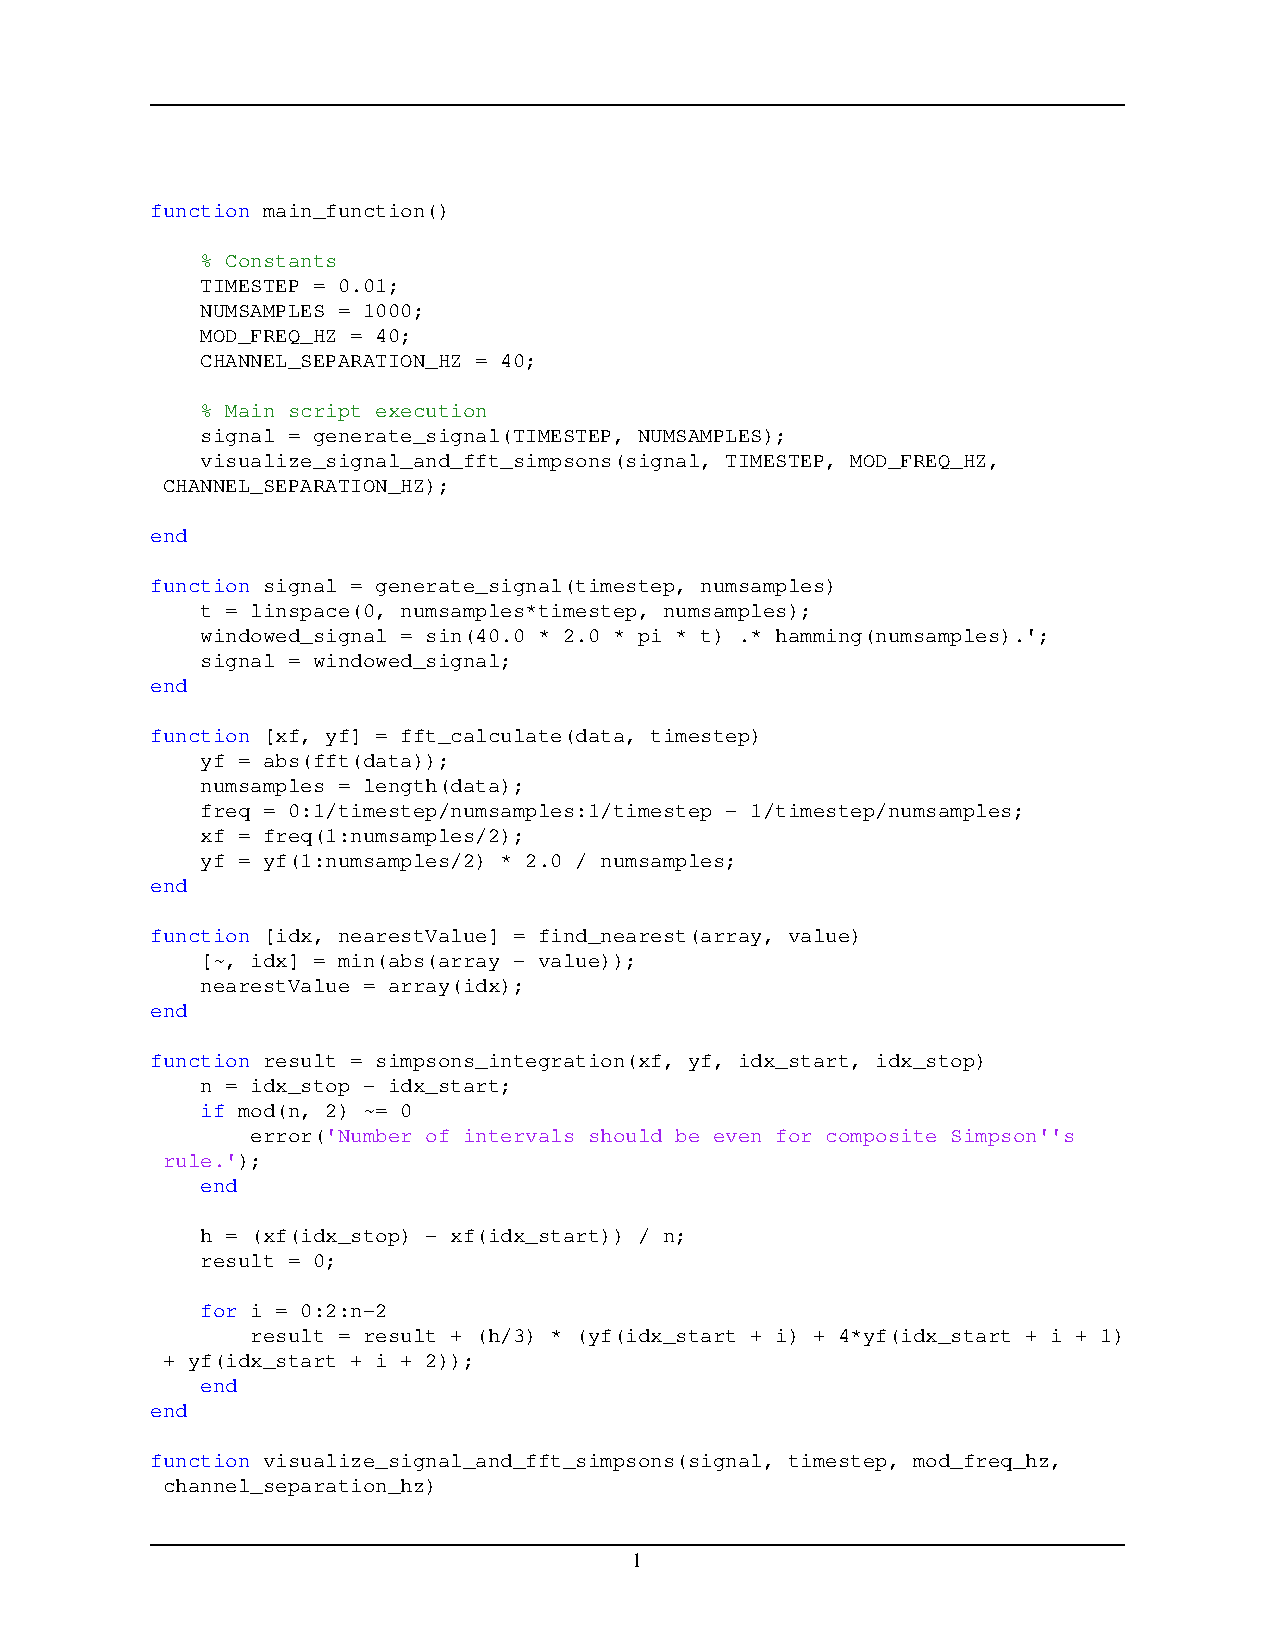
\includepdf[pages=-]{matlab_outputs/a1.pdf} % Include the MATLAB PDF
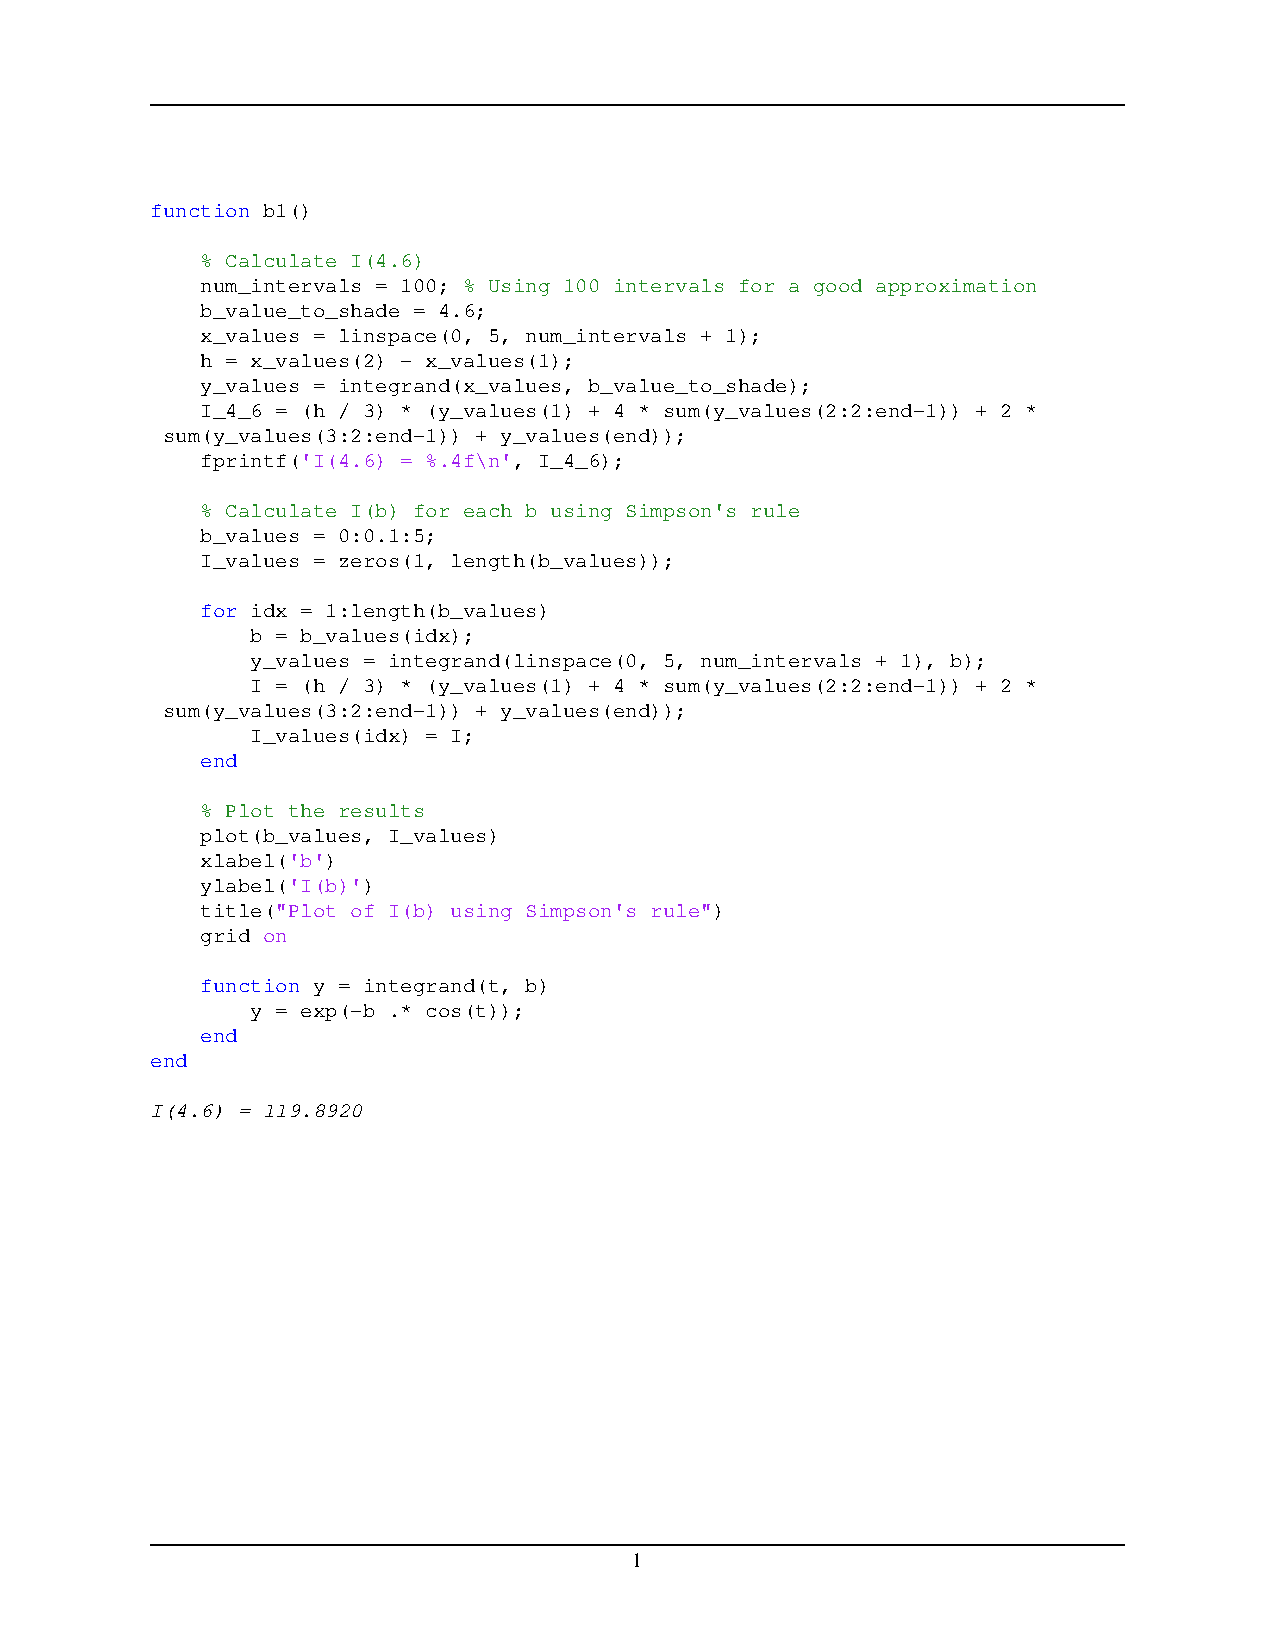
\includepdf[pages=-]{matlab_outputs/b1.pdf} % Include the MATLAB PDF
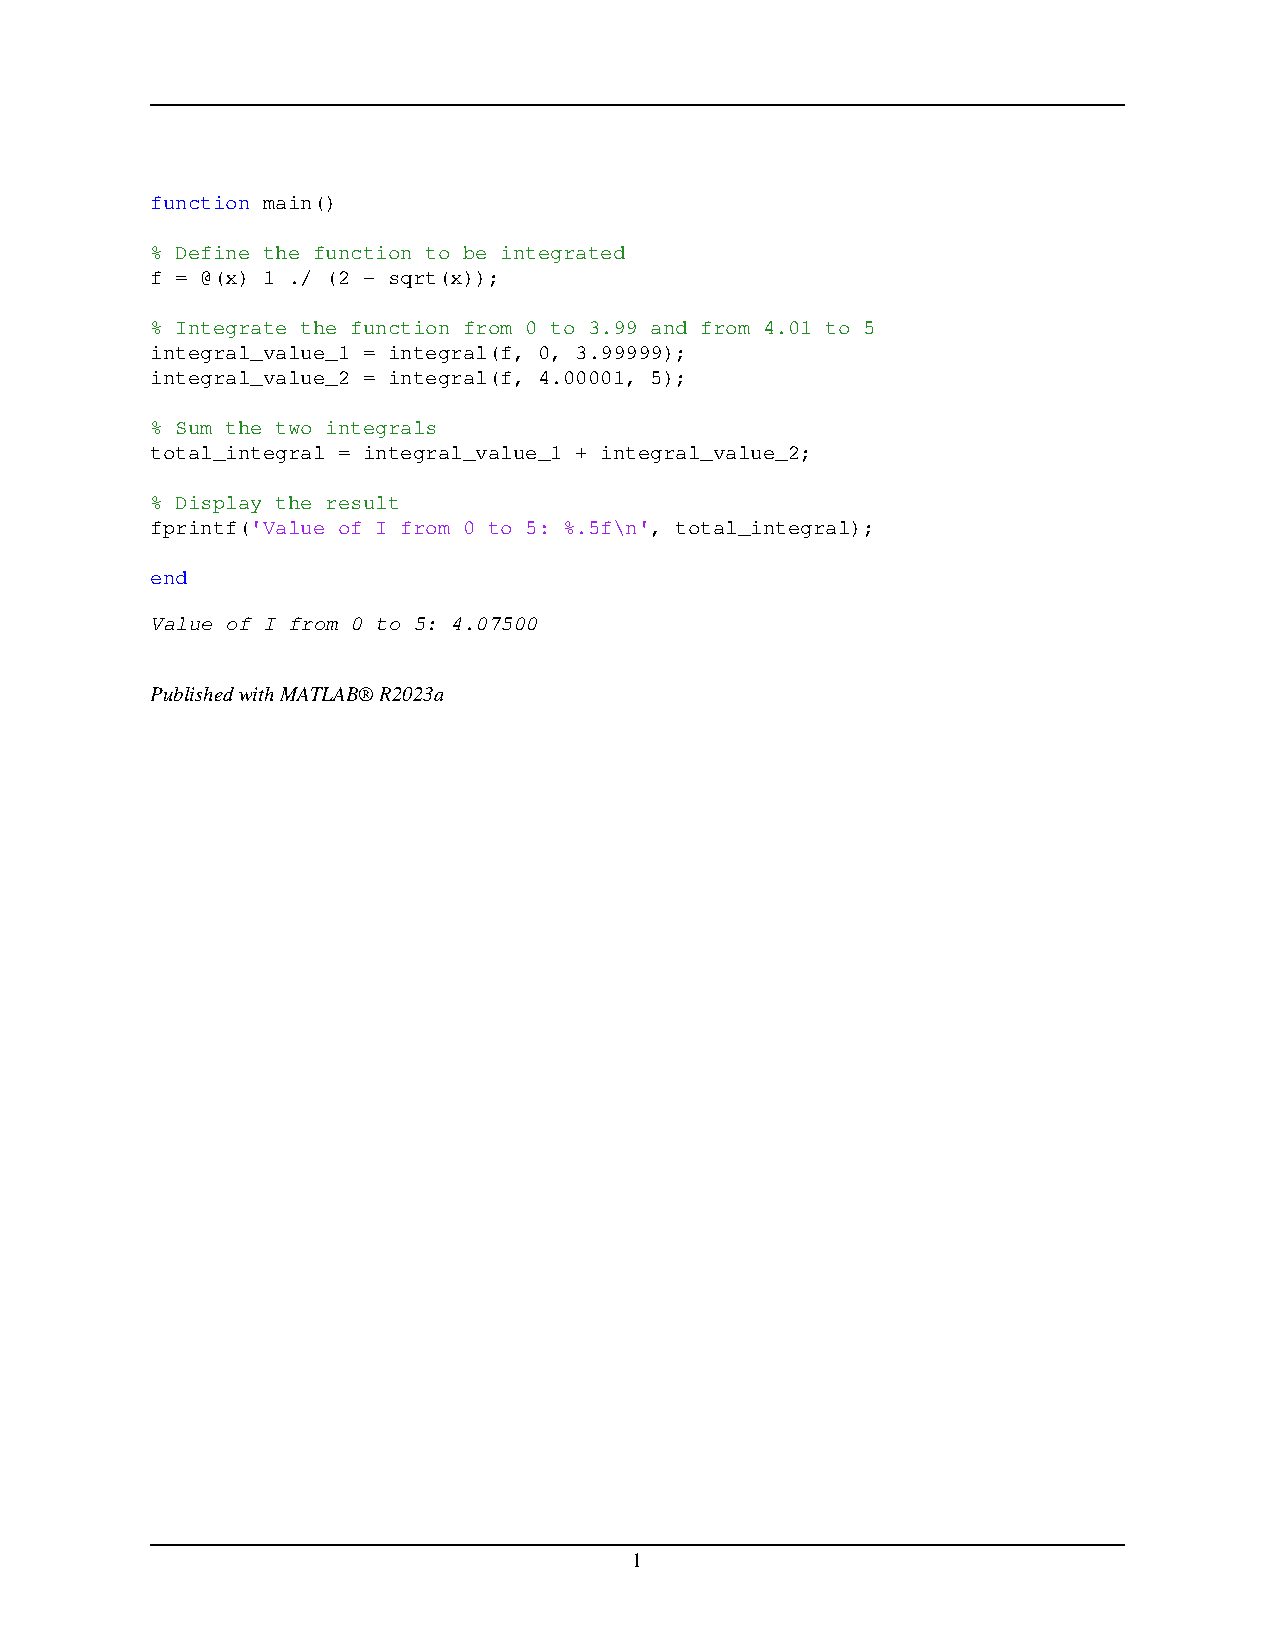
\includepdf[pages=-]{matlab_outputs/c1.pdf} % Include the MATLAB PDF
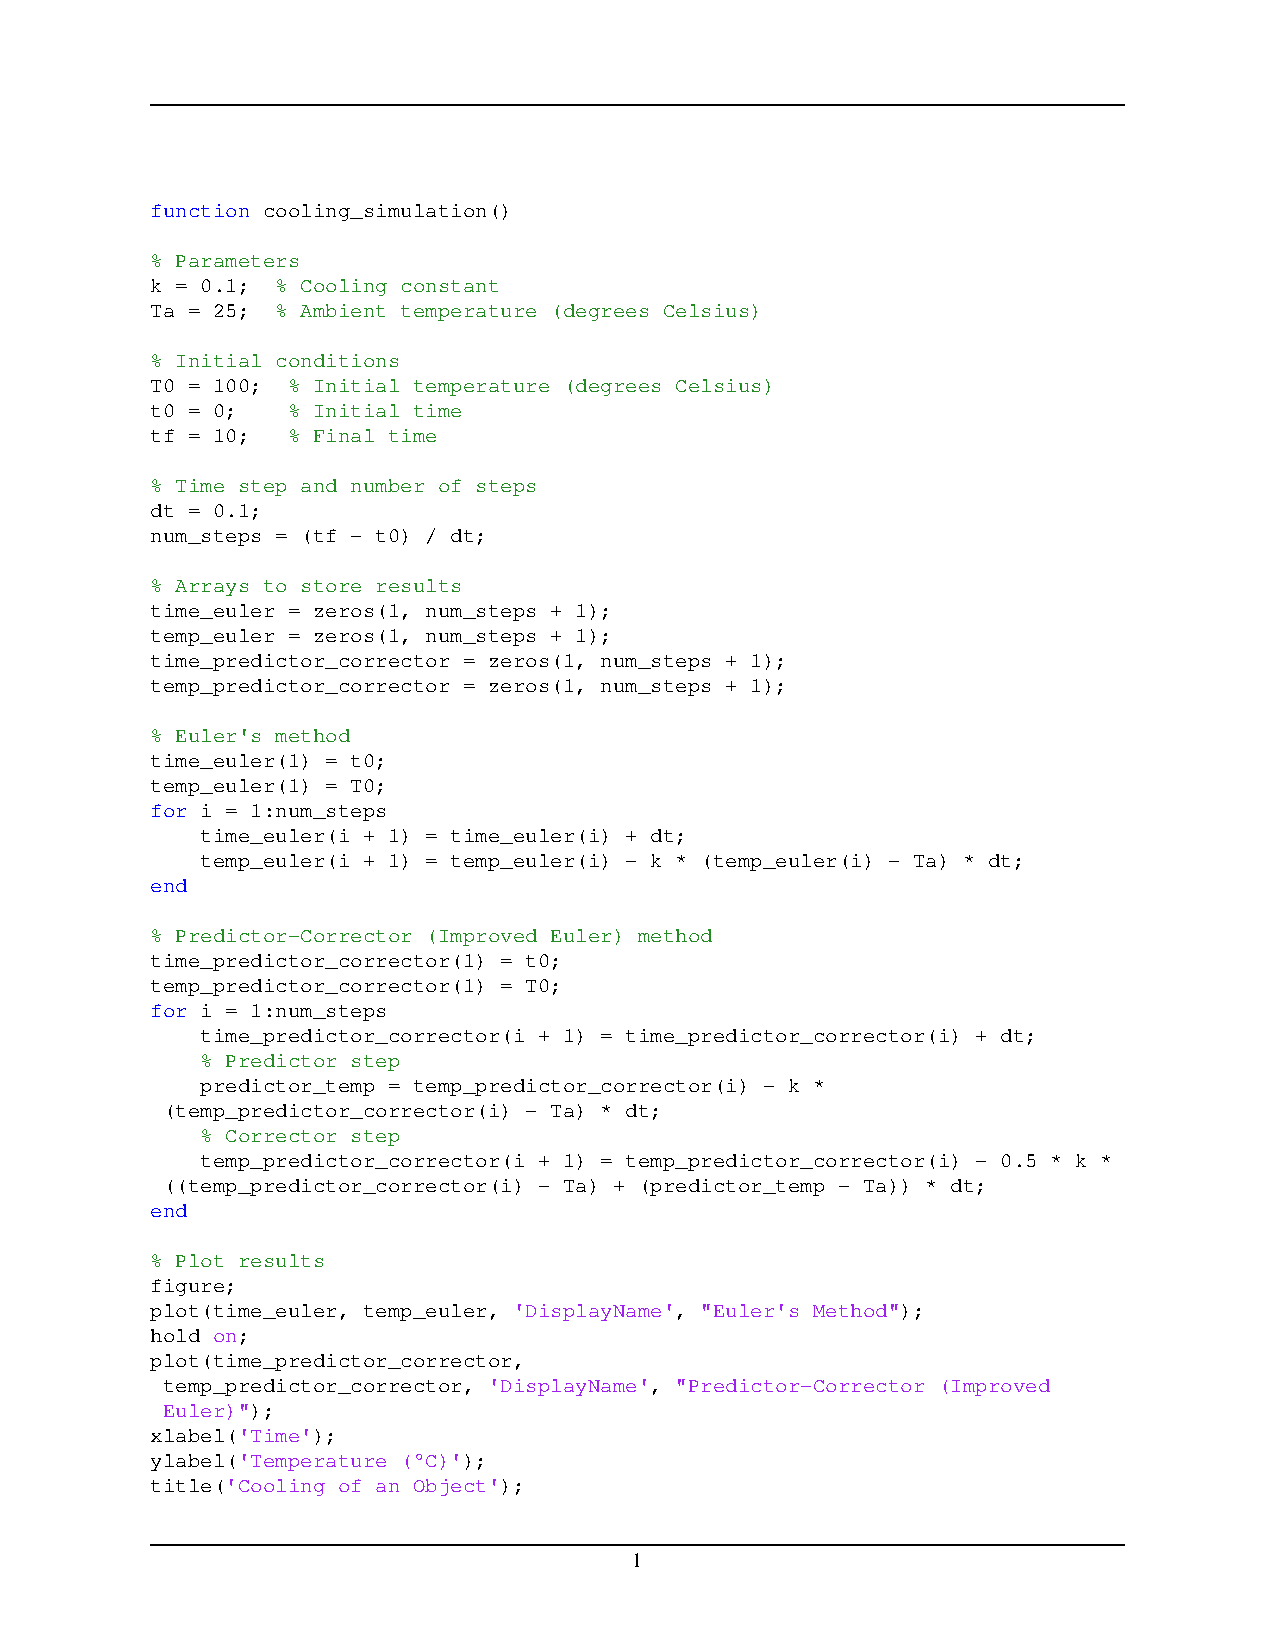
\includepdf[pages=-]{matlab_outputs/a2.pdf} % Include the MATLAB PDF
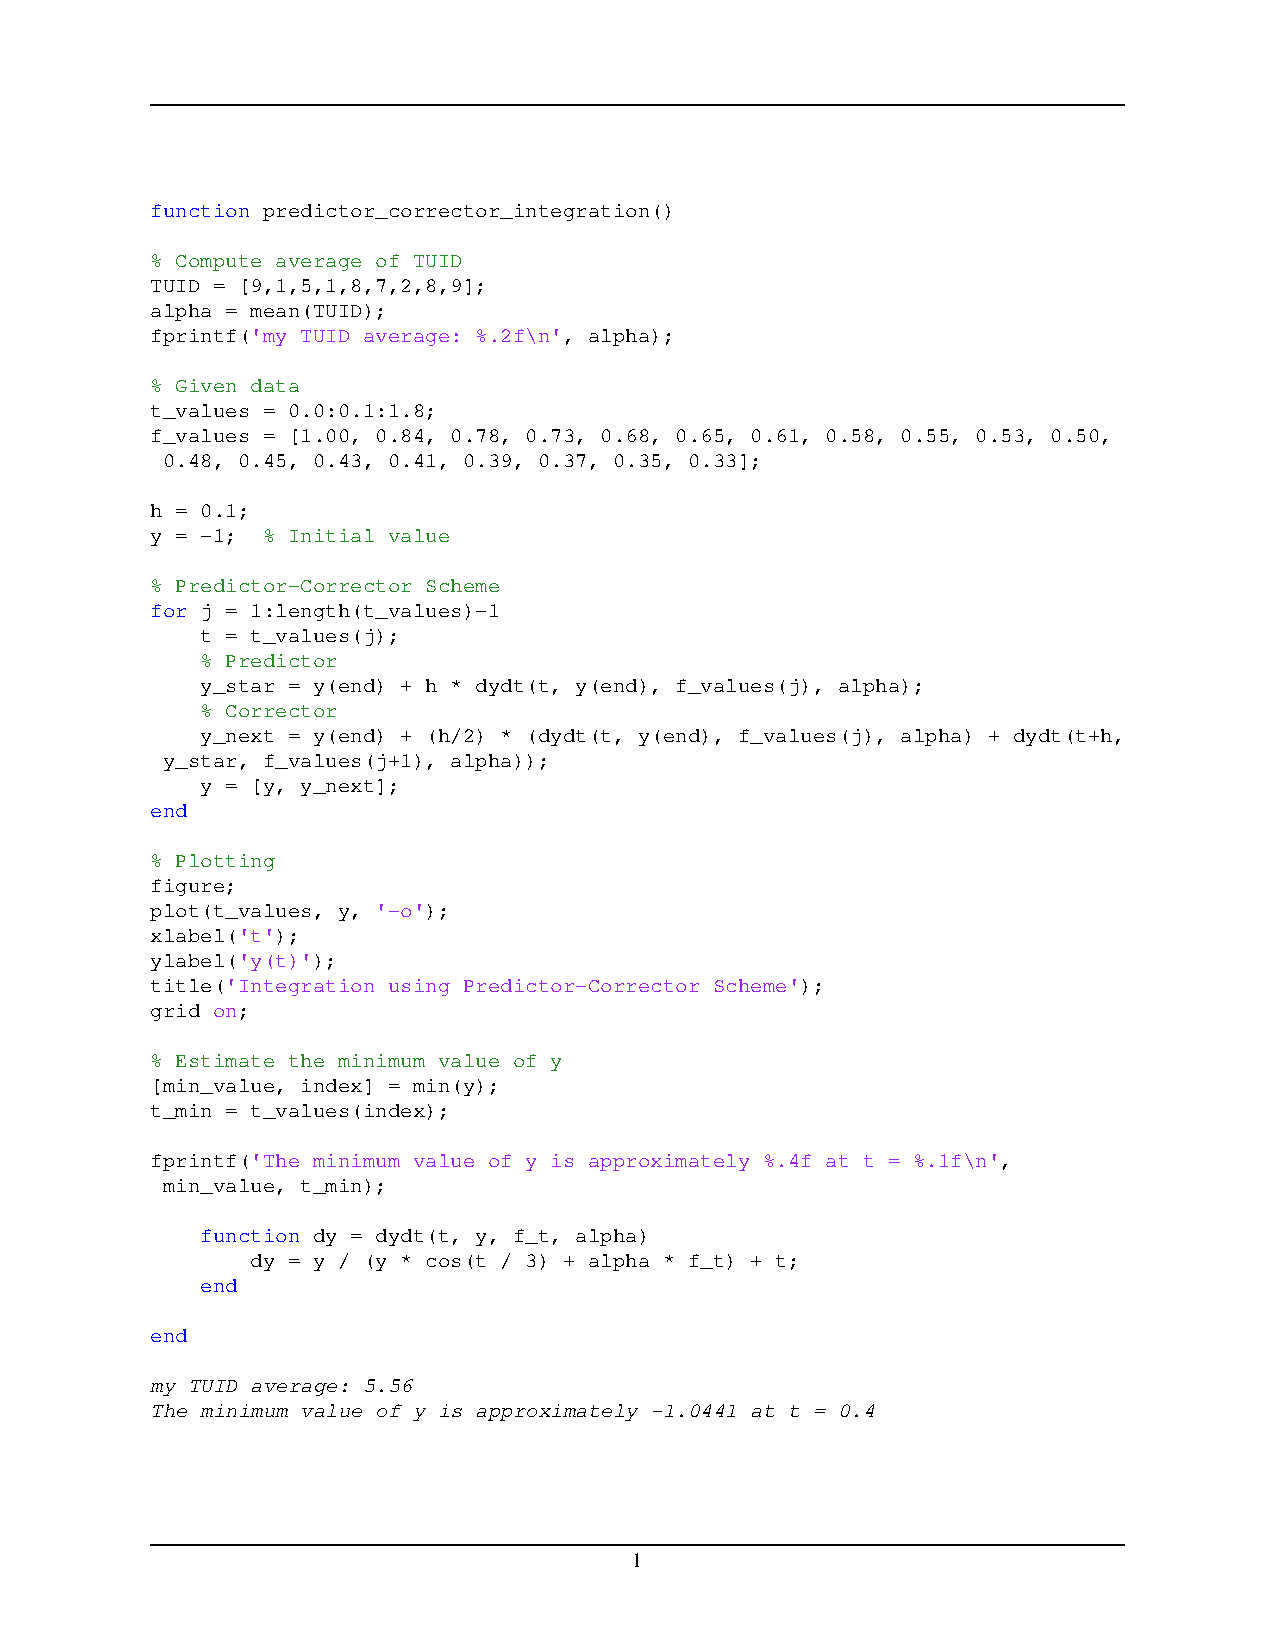
\includepdf[pages=-]{matlab_outputs/b2.pdf} % Include the MATLAB PDF
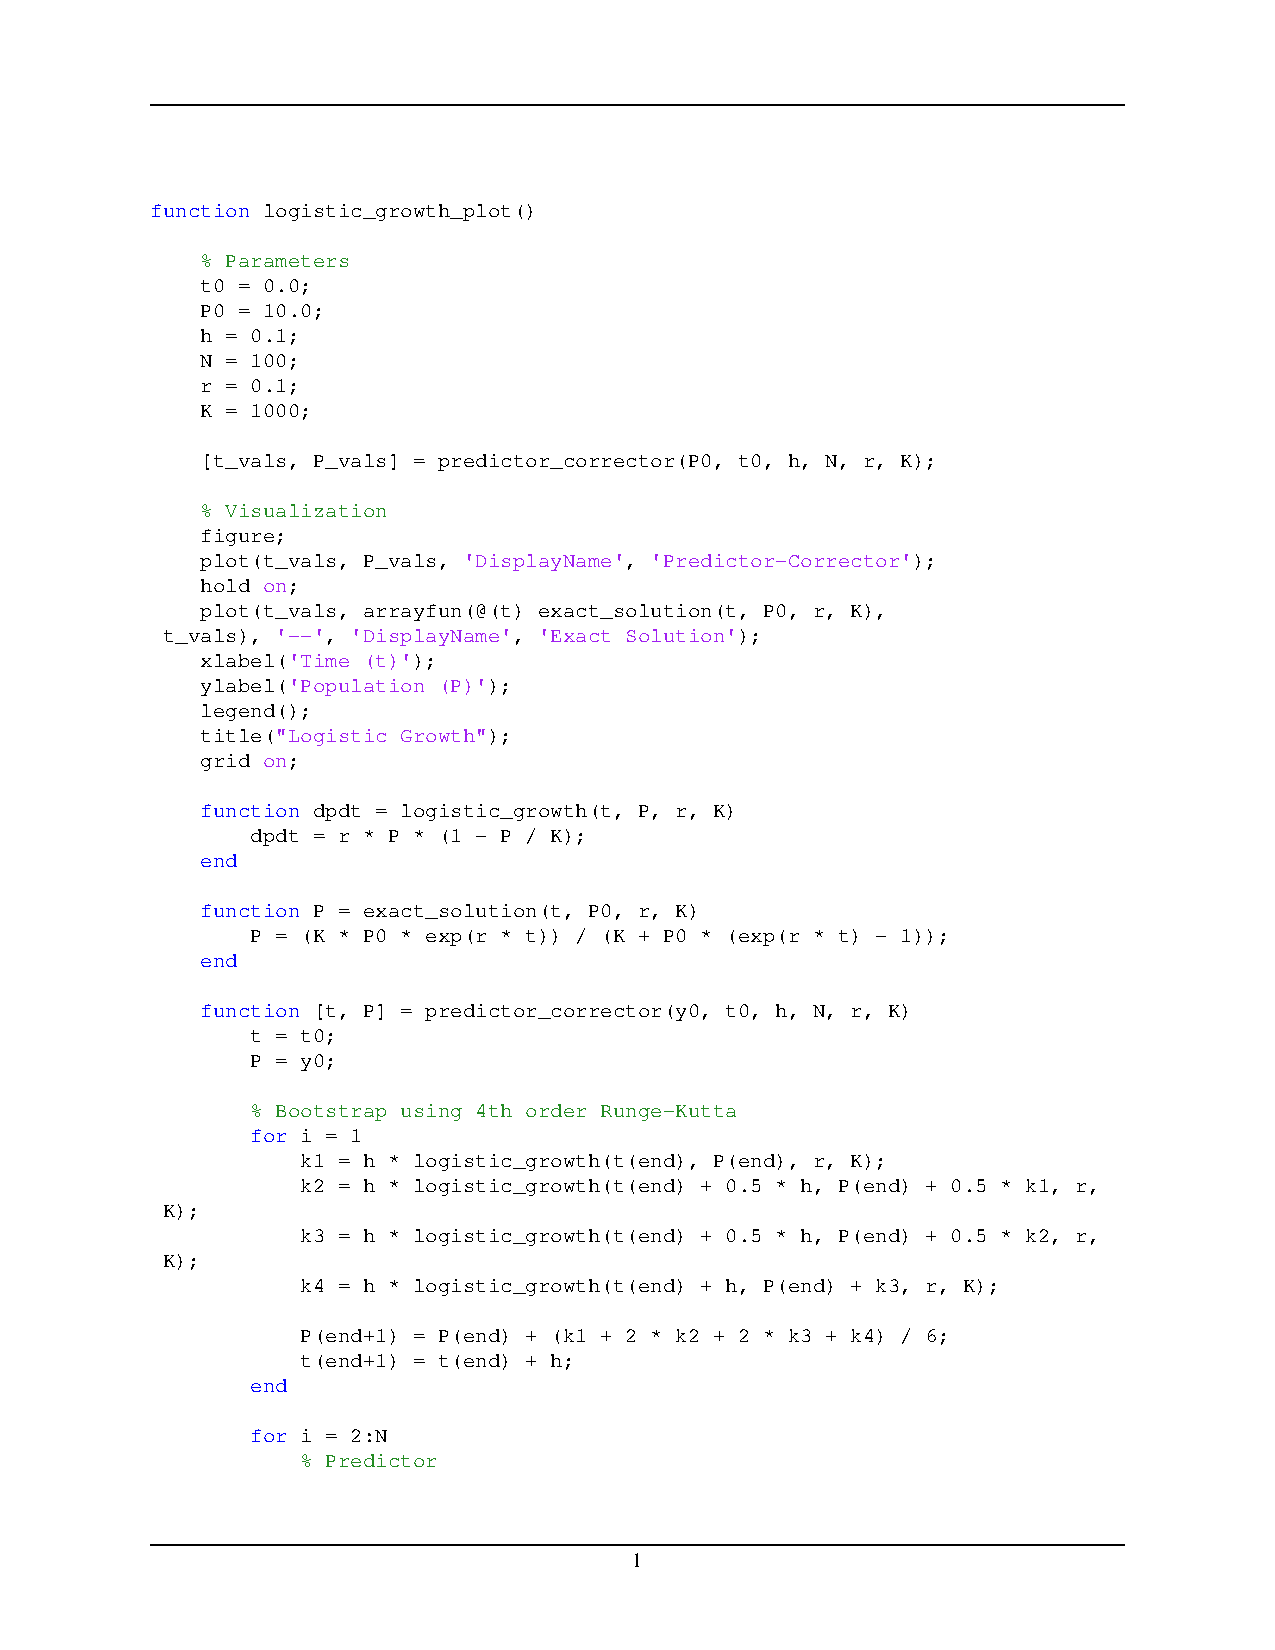
\includepdf[pages=-]{matlab_outputs/a3.pdf} % Include the MATLAB PDF
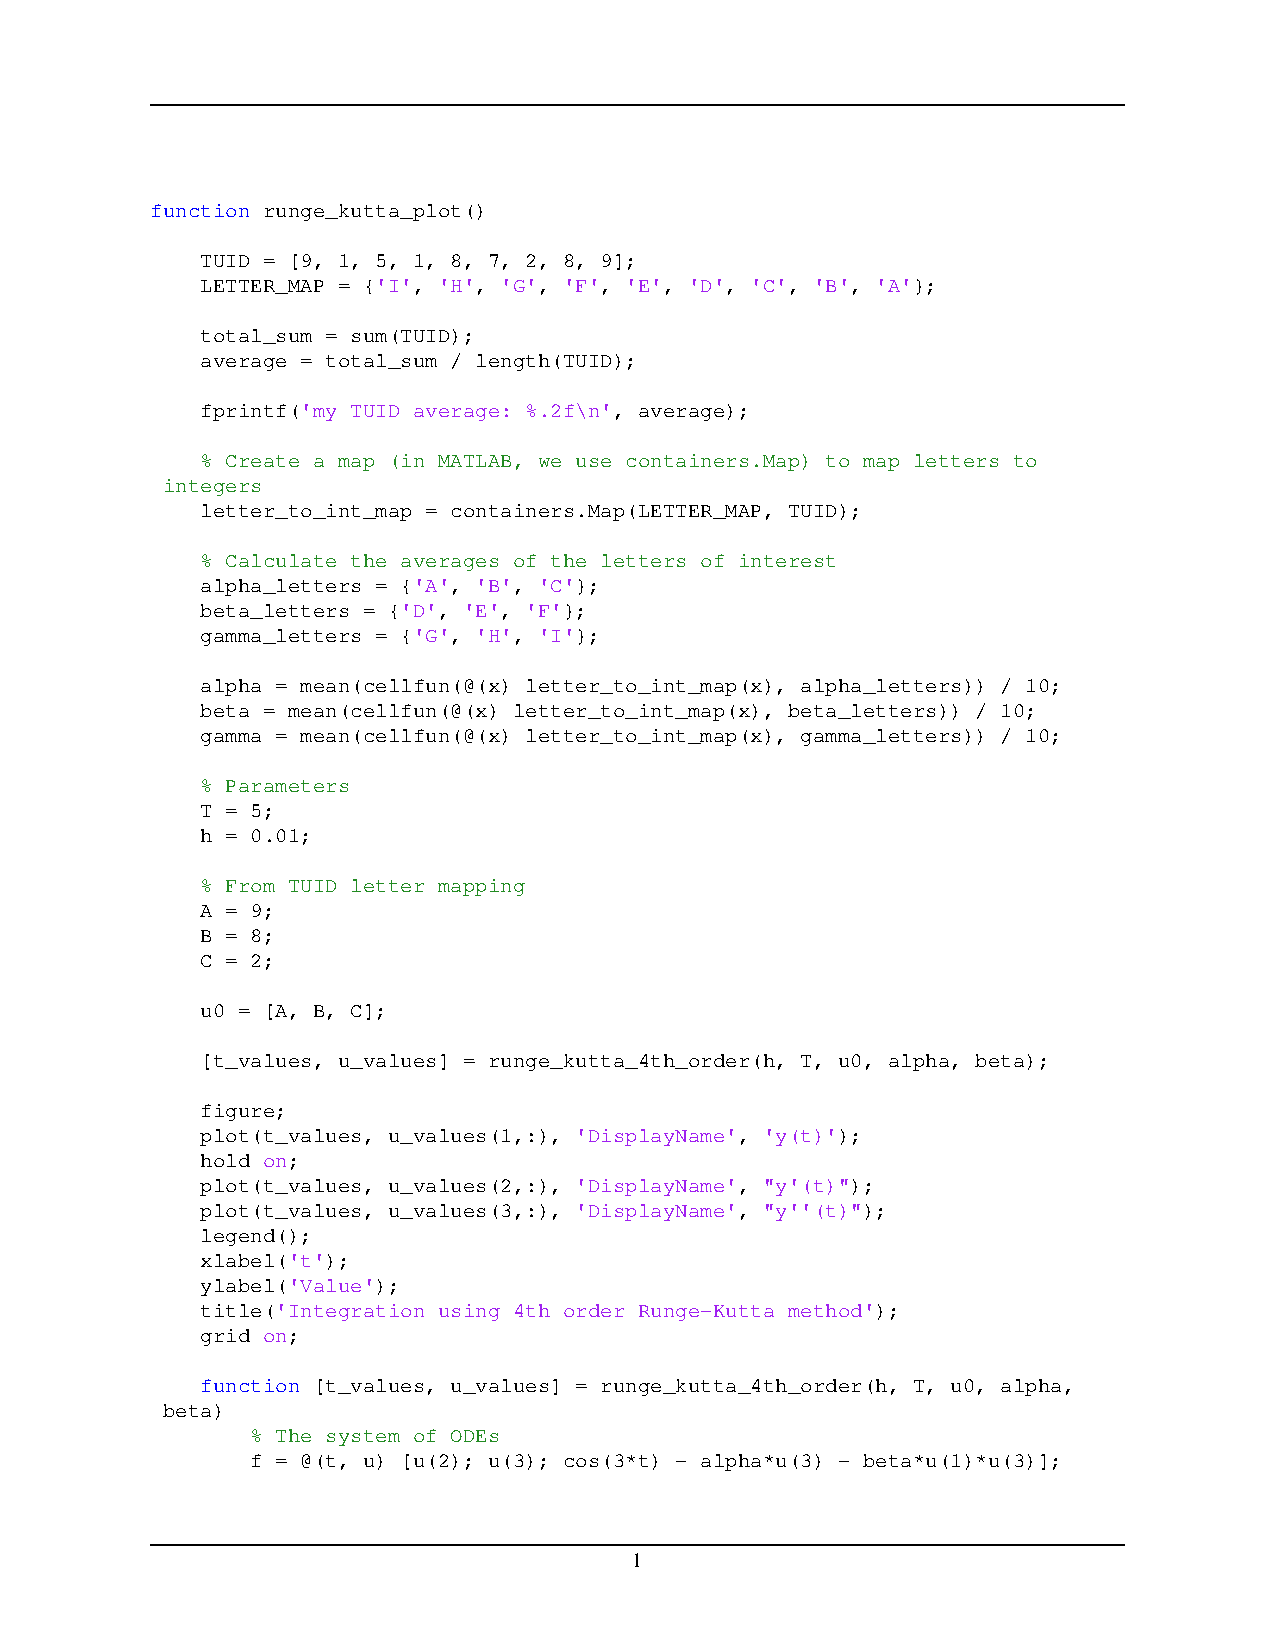
\includepdf[pages=-]{matlab_outputs/b3.pdf} % Include the MATLAB PDF

\section{Compiled Plots}

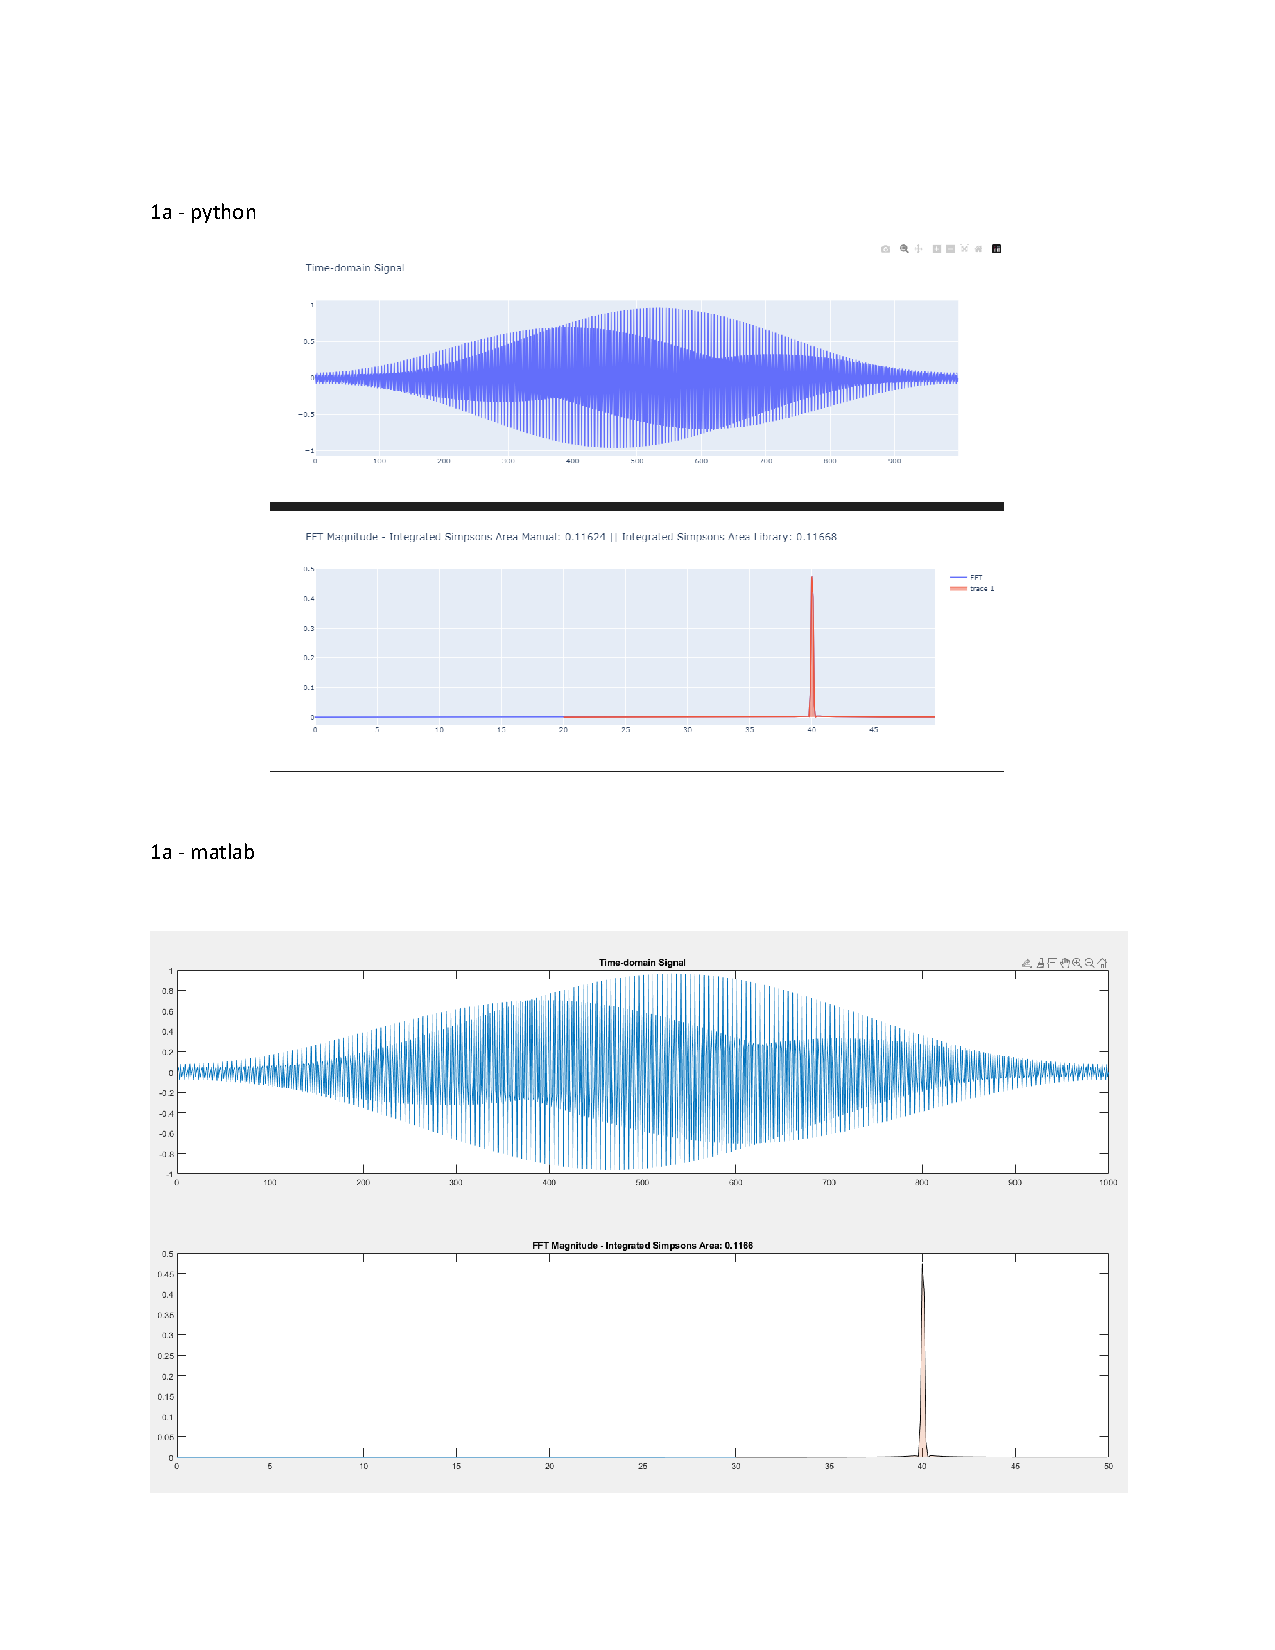
\includepdf[pages=-]{compiled_outputs/compiled_plots.pdf} % Include the Python PDF

\end{document}
